% ============================================================
% Modul 03: NLP Fundamentals
% Custom Navasena Dark Beamer Theme
% Compiler: xelatex
% ============================================================
\documentclass[aspectratio=169,t]{beamer}

% ---- Fonts (xelatex) ----------------------------------------
\usepackage{fontspec}
\usepackage[sfdefault]{FiraSans}

% ---- Core packages ------------------------------------------
\usepackage{graphicx}
\usepackage{tikz}
\usetikzlibrary{positioning, shapes.geometric, arrows.meta, calc}
\usepackage{pgfplots}
\pgfplotsset{compat=1.18}
\usepackage{amsmath}
\usepackage{booktabs}
\usepackage{colortbl}
\usepackage{xcolor}
\usepackage{listings}
\usepackage{pifont}

% ============================================================
% COLOR PALETTE (Navasena dark theme)
% ============================================================
\definecolor{nvbg}{HTML}{1A1A2E}        % dark navy background
\definecolor{nvdark}{HTML}{1A1A2E}     % alias for nvbg
\definecolor{nvcard}{HTML}{2D2D44}      % card / box background
\definecolor{nvgreen}{HTML}{76B900}     % primary accent
\definecolor{nvlightgreen}{HTML}{A3D944}% secondary accent
\definecolor{nvwhite}{HTML}{FFFFFF}
\definecolor{nvgray}{HTML}{AAAACC}      % muted text
\definecolor{nvdarkcard}{HTML}{23233A}  % slightly darker card
\definecolor{nvred}{HTML}{EF5350}       % accent red
\definecolor{nvorange}{HTML}{FF6F00}    % accent orange
\definecolor{nvblue}{HTML}{42A5F5}      % accent blue (for ID/EN distinction)

% ============================================================
% LISTINGS STYLE
% ============================================================
\lstset{
  backgroundcolor=\color{nvcard},
  basicstyle=\ttfamily\small\color{nvwhite},
  keywordstyle=\color{nvgreen}\bfseries,
  stringstyle=\color{nvlightgreen},
  commentstyle=\color{nvgray}\itshape,
  numberstyle=\tiny\color{nvgray},
  numbers=left,
  numbersep=6pt,
  frame=none,
  breaklines=true,
  showstringspaces=false,
  tabsize=2,
  xleftmargin=8pt,
  xrightmargin=4pt,
}

% ============================================================
% BEAMER THEME — NAVASENA DARK
% ============================================================
\usetheme{default}
\usecolortheme{default}

% Background
\setbeamercolor{background canvas}{bg=nvbg}
\setbeamercolor{normal text}{fg=nvwhite}

% Frames
\setbeamercolor{frametitle}{fg=nvwhite, bg=nvbg}
\setbeamercolor{framesubtitle}{fg=nvgray, bg=nvbg}
\setbeamercolor{title}{fg=nvgreen}
\setbeamercolor{author}{fg=nvgray}
\setbeamercolor{date}{fg=nvgray}
\setbeamercolor{item}{fg=nvgreen}
\setbeamercolor{subitem}{fg=nvlightgreen}
\setbeamercolor{subsubitem}{fg=nvgray}
\setbeamercolor{block title}{fg=nvwhite, bg=nvcard}
\setbeamercolor{block body}{fg=nvwhite, bg=nvcard}

% Footline
\setbeamertemplate{footline}{%
  \hbox{%
    \begin{beamercolorbox}[wd=\paperwidth,ht=2.5ex,dp=1ex,leftskip=2em]{author in head/foot}%
      \color{nvgray}\small\textbf{NLP Fundamentals} \hfill \insertframenumber\,/\,\inserttotalframenumber
    \end{beamercolorbox}%
  }%
}

% Remove nav symbols
\setbeamertemplate{navigation symbols}{}

% ============================================================
% CUSTOM COMMANDS
% ============================================================
% \acttitle{Act N}{Title}{Subtitle/question}
\newcommand{\acttitle}[3]{%
  \begin{frame}[plain]
    \vspace{1.5cm}
    \begin{center}
      {\color{nvgreen}\Huge\bfseries Act #1}\\[1.2em]
      {\color{nvwhite}\Huge #2}\\[0.8em]
      {\color{nvgray}\Large #3}
    \end{center}
  \end{frame}%
}

% Section divider
\newcommand{\sectiontitle}[2]{%
  \begin{frame}[plain]
    \vspace{2cm}
    \begin{center}
      {\color{nvgreen}\Huge\bfseries #1}\\[1em]
      {\color{nvgray}\Large #2}
    \end{center}
  \end{frame}%
}

% Kotak info berwarna: \nvbox{Judul}{isi}
\newcommand{\nvbox}[2]{%
  \begin{tikzpicture}
    \node[fill=nvcard, rounded corners=4pt, inner sep=8pt,
          text width=\linewidth-16pt, text=nvwhite]
      {\textbf{\color{nvgreen}#1}\\\medskip#2};
  \end{tikzpicture}%
}

% \intuisi{Judul} -> frametitle "Judul" + tag kecil "Intuisi" di kanan atas
\newcommand{\intuisi}[1]{%
  \frametitle{\makebox[\dimexpr\paperwidth-1.7cm\relax][l]{%
    #1\hfill{\small\color{nvlightgreen}Intuisi}}}}

% \jebakan{teks} -> kotak oranye
\newcommand{\jebakan}[1]{%
  \begin{tikzpicture}
    \node[fill=nvorange!25!nvbg, draw=nvorange, rounded corners=4pt, inner sep=7pt,
          text width=\linewidth-16pt, text=nvwhite]
      {\textbf{\color{nvorange}Jebakan:} #1};
  \end{tikzpicture}%
}

% \kapan{cocok}{kurang cocok} -> dua kolom hijau/merah
\newcommand{\kapan}[2]{%
  \begin{columns}[T]
    \begin{column}{0.48\textwidth}
      \textbf{\color{nvgreen}Cocok kalau}
      \begin{itemize}#1\end{itemize}
    \end{column}
    \begin{column}{0.48\textwidth}
      \textbf{\color{nvred}Kurang cocok kalau}
      \begin{itemize}#2\end{itemize}
    \end{column}
  \end{columns}%
}

% Title page

\title{NLP Fundamentals}
\subtitle{Navasena Gen-ML Course}
\author{Navasena AI}
\date{}

% ============================================================
% DOCUMENT START
% ============================================================
\begin{document}

% ── Title slide ────────────────────────────────────────────
\begin{frame}[plain]
  \vspace{1.2cm}
  \begin{center}
    {\color{nvgreen}\Huge\bfseries Modul 03}\\[1.2em]
    {\color{nvwhite}\Huge\bfseries NLP Fundamentals}\\[0.6em]
    {\color{nvgray}\Large Natural Language Processing dengan Python}\\[2.5em]

    \begin{tikzpicture}[scale=0.85]
      % Central brain icon
      \node[circle, fill=nvcard, draw=nvgreen, line width=2pt,
            minimum size=1.8cm, align=center] (brain) at (0,0)
            {\color{nvwhite}\Large\bfseries NLP};
      % Surrounding language labels
      \node[color=nvgray, font=\small] at (-2.5,1.0) {EN};
      \node[color=nvgray, font=\small] at (2.5,1.0) {中文};
      \node[color=nvgray, font=\small] at (-2.5,-1.0) {ID};
      \node[color=nvgray, font=\small] at (2.5,-1.0) {ES};
      \draw[->,color=nvgreen,thin] (-2.2,0.85) to[bend left=15] (-0.9,0.25);
      \draw[->,color=nvgreen,thin] (2.2,0.85) to[bend right=15] (0.9,0.25);
      \draw[->,color=nvgreen,thin] (-2.2,-0.85) to[bend right=15] (-0.9,-0.25);
      \draw[->,color=nvgreen,thin] (2.2,-0.85) to[bend left=15] (0.9,-0.25);
    \end{tikzpicture}

    \vspace{0.8em}
    {\color{nvgray}\small Navasena AI \quad $\cdot$ \quad 2026}
  \end{center}
\end{frame}

% ============================================================
% ACT 1 — APA ITU NLP
% ============================================================
\acttitle{1}{Apa itu NLP?}{Bagaimana komputer memahami bahasa manusia?}

\begin{frame}{Definisi NLP}
  \begin{columns}[T]
    \begin{column}{0.55\textwidth}
      \begin{itemize}
        \item \textbf{Natural Language Processing}
        \item Cabang AI yang membuat komputer \textbf{memahami} \& \textbf{memproses} bahasa manusia
        \item Bukan sekadar manipulasi string
        \item[\textcolor{nvgreen}{\checkmark}] Bahasa: Inggris, Indonesia, Mandarin, dll
        \item[\textcolor{nvgreen}{\checkmark}] Bentuk: teks, suara
      \end{itemize}
      \vspace{0.5em}
      \begin{beamercolorbox}[rounded=true,shadow=false,sep=4pt]{block body}
        \small\color{white}
        Contoh: Google Translate, Siri, ChatGPT, mesin pencari
      \end{beamercolorbox}
    \end{column}
    \begin{column}{0.42\textwidth}
      \begin{center}
      \resizebox{\linewidth}{!}{%
      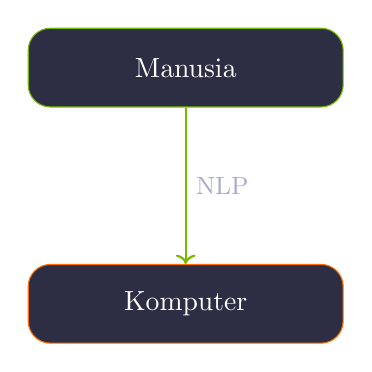
\begin{tikzpicture}
        \node[draw=nvgreen, fill=nvcard, rounded corners=8pt,
              minimum width=4cm, minimum height=1cm, align=center,
              text=white] (hum) at (0,3) {Manusia};
        \node[draw=nvorange, fill=nvcard, rounded corners=8pt,
              minimum width=4cm, minimum height=1cm, align=center,
              text=white] (com) at (0,0) {Komputer};
        \draw[->,thick,color=nvgreen] (hum) -- (com)
          node[midway, right, color=nvgray, font=\small] {NLP};
      \end{tikzpicture}%
      }
      \end{center}
    \end{column}
  \end{columns}
\end{frame}

\begin{frame}{Aplikasi NLP di Dunia Nyata}
  \begin{itemize}
    \item[\textcolor{nvgreen}{\checkmark}] \textbf{Mesin pencari} (Google, Bing) $\to$ memahami maksud query
    \item[\textcolor{nvgreen}{\checkmark}] \textbf{Penerjemahan mesin} (Google Translate) $\to$ lintas bahasa
    \item[\textcolor{nvgreen}{\checkmark}] \textbf{Analisis sentimen} $\to$ ulasan produk, pemantauan merek
    \item[\textcolor{nvgreen}{\checkmark}] \textbf{Chatbot \& asisten} (Siri, Alexa) $\to$ percakapan
    \item[\textcolor{nvgreen}{\checkmark}] \textbf{Klasifikasi teks} $\to$ penyaring spam, kategorisasi berita
    \item[\textcolor{nvgreen}{\checkmark}] \textbf{Peringkasan} $\to$ ringkasan otomatis dokumen
  \end{itemize}
  \vspace{0.5em}
  \begin{center}
    
\begin{tikzpicture}
      \node[draw=nvgreen, fill=nvcard, rounded corners=4pt,
            text=white, font=\small\bfseries, minimum width=2cm, minimum height=0.6cm] (a) at (0,0) {Teks};
      \node[draw=nvorange, fill=nvcard, rounded corners=4pt,
            text=white, font=\small\bfseries, minimum width=2cm, minimum height=0.6cm] (b) at (3.2,0) {Keputusan};
      \draw[->,thick,color=nvgreen] (a) -- (b);
    \end{tikzpicture}
  \end{center}
\end{frame}

\begin{frame}{Tantangan Bahasa Manusia}
  \begin{columns}[T]
    \begin{column}{0.5\textwidth}
      \textcolor{nvblue}{\textbf{Bahasa Inggris:}}\\
      \begin{itemize}
        \footnotesize
        \item Morfologi sederhana\\
              \texttt{run $\to$ runs $\to$ running}
        \item Urutan kata tetap (SVO)
        \item Imbuhan terbatas (\texttt{-s, -ed, -ing})
      \end{itemize}
    \end{column}
    \begin{column}{0.5\textwidth}
      \textcolor{nvorange}{\textbf{Bahasa Indonesia:}}\\
      \begin{itemize}
        \footnotesize
        \item Imbuhan kaya\\
              \texttt{jalan $\to$ menjalani $\to$ dijalankan}
        \item Imbuhan: \texttt{me-, -kan, -i, pe-, -an, ber-}
        \item Kata serapan dan singkatan
      \end{itemize}
    \end{column}
  \end{columns}
  \vspace{1em}
  \begin{beamercolorbox}[rounded=true,shadow=false,sep=6pt]{block body}
    \centering
    \small\color{nvlightgreen}
    Bahasa berbeda butuh library berbeda: \texttt{nltk + spaCy} untuk Inggris,
    \texttt{nlp-id} untuk Indonesia
  \end{beamercolorbox}
\end{frame}

\begin{frame}
  \intuisi{Satu kata dasar, belasan bentuk permukaan}
  \vspace{0.3em}
  \begin{center}
  \resizebox{0.86\linewidth}{!}{%
  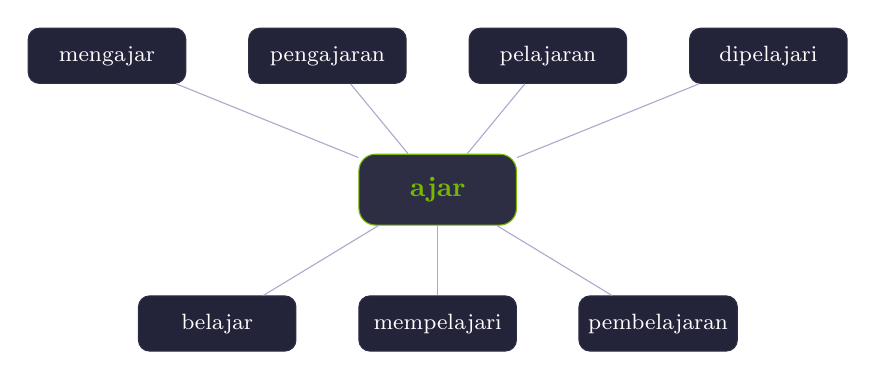
\begin{tikzpicture}[font=\small]
    \node[draw=nvgreen, fill=nvcard, rounded corners=6pt, text=nvgreen,
          font=\bfseries, minimum width=2cm, minimum height=0.9cm] (root) at (0,0) {ajar};
    \foreach \x/\y/\w in {-4.2/1.7/mengajar, -1.4/1.7/pengajaran, 1.4/1.7/pelajaran,
                          4.2/1.7/dipelajari, -2.8/-1.7/belajar, 0/-1.7/mempelajari,
                          2.8/-1.7/pembelajaran}{
      \node[draw=nvcard, fill=nvdarkcard, rounded corners=4pt, text=nvwhite,
            font=\footnotesize, minimum width=2cm, minimum height=0.7cm] (n\w) at (\x,\y) {\w};
      \draw[nvgray, thin] (root) -- (n\w);
    }
  \end{tikzpicture}%
  }
  \end{center}
  \vspace{0.3em}
  \begin{center}
    {\color{nvlightgreen}\small Mesin melihat tujuh kata berbeda. Manusia melihat satu gagasan.
    Lemmatisasi adalah usaha menutup jarak itu.}
  \end{center}
\end{frame}

\begin{frame}{Peta Perjalanan Modul 03}
  \begin{center}
  \resizebox{0.95\linewidth}{!}{%
  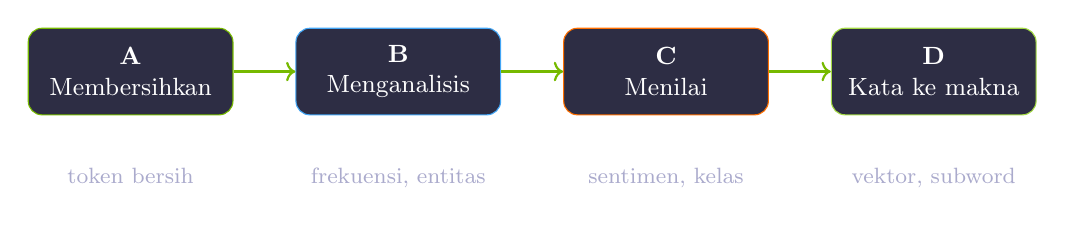
\begin{tikzpicture}[font=\small, node distance=0.4cm]
    \node[draw=nvgreen, fill=nvcard, rounded corners=5pt, text=nvwhite,
          minimum width=2.6cm, minimum height=1.1cm, align=center] (a) at (0,0)
          {\textbf{A}\\Membersihkan};
    \node[draw=nvblue, fill=nvcard, rounded corners=5pt, text=nvwhite,
          minimum width=2.6cm, minimum height=1.1cm, align=center] (b) at (3.4,0)
          {\textbf{B}\\Menganalisis};
    \node[draw=nvorange, fill=nvcard, rounded corners=5pt, text=nvwhite,
          minimum width=2.6cm, minimum height=1.1cm, align=center] (c) at (6.8,0)
          {\textbf{C}\\Menilai};
    \node[draw=nvlightgreen, fill=nvcard, rounded corners=5pt, text=nvwhite,
          minimum width=2.6cm, minimum height=1.1cm, align=center] (d) at (10.2,0)
          {\textbf{D}\\Kata ke makna};
    \foreach \s/\t in {a/b, b/c, c/d} \draw[->,thick,color=nvgreen] (\s) -- (\t);
    \node[text=nvgray, font=\footnotesize, below=0.55cm of a] {token bersih};
    \node[text=nvgray, font=\footnotesize, below=0.55cm of b] {frekuensi, entitas};
    \node[text=nvgray, font=\footnotesize, below=0.55cm of c] {sentimen, kelas};
    \node[text=nvgray, font=\footnotesize, below=0.55cm of d] {vektor, subword};
  \end{tikzpicture}%
  }
  \end{center}
  \vspace{0.8em}
  \begin{itemize}
    \footnotesize
    \item Notebook 01 menempuh keempat bagian di CPU
    \item Notebook 02 mengulang alur yang sama di GPU dengan NVIDIA RAPIDS
    \item Bagian D adalah jembatan langsung ke Modul 04 (LLM) dan Modul 05 (RAG)
  \end{itemize}
\end{frame}

% ============================================================
% ACT 2 — MEMBERSIHKAN TEKS
% ============================================================
\acttitle{2}{Membersihkan Teks}{Kenapa langkah paling membosankan justru paling menentukan}

\begin{frame}{Pipeline NLP: Dari Teks ke Model}
  \begin{center}
    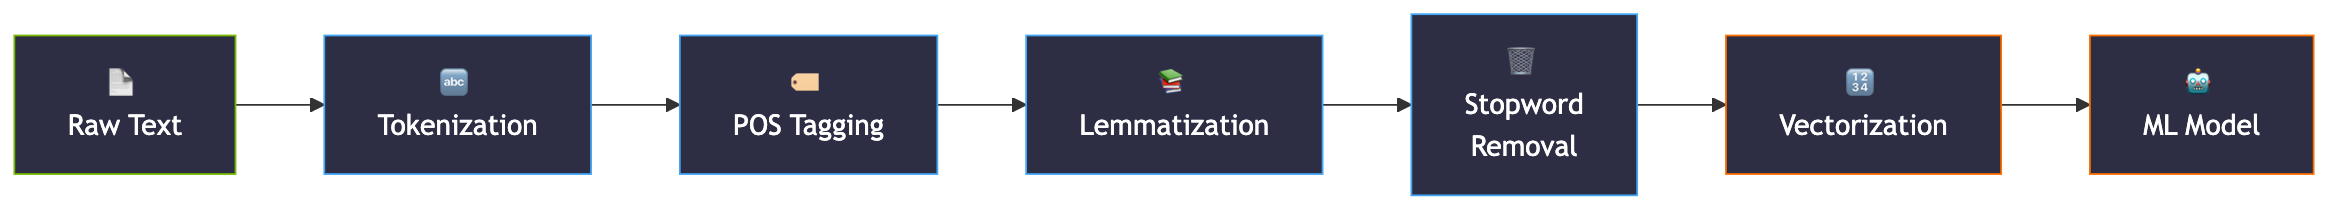
\includegraphics[width=0.85\textwidth]{figures/nlp_pipeline.png}
  \end{center}
  \vspace{0.3em}
  \begin{center}
    \textcolor{nvlightgreen}{\small Tahapan utama: dari teks mentah sampai siap masuk model ML}
  \end{center}
\end{frame}

\begin{frame}{Tokenisasi: Memecah Teks}
  \begin{columns}[T]
    \begin{column}{0.48\textwidth}
      \begin{center}
      \resizebox{\linewidth}{!}{%
      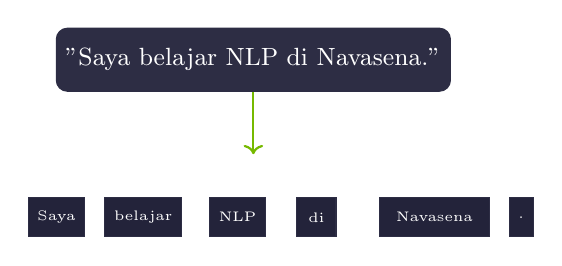
\begin{tikzpicture}
        \node[draw=nvcard, fill=nvcard, rounded corners=4pt,
              text=white, font=\small, align=center,
              minimum width=5cm, minimum height=0.8cm] (raw) at (0,0)
              {"Saya belajar NLP di Navasena."};
        \draw[->,thick,color=nvgreen] (raw) -- (0,-1.2);
        \node[draw=nvcard, fill=nvdarkcard, text=nvwhite, font=\tiny,
              minimum width=0.6cm, minimum height=0.5cm] (t1) at (-2.5,-2.0) {Saya};
        \node[draw=nvcard, fill=nvdarkcard, text=nvwhite, font=\tiny,
              minimum width=0.8cm, minimum height=0.5cm] (t2) at (-1.4,-2.0) {belajar};
        \node[draw=nvcard, fill=nvdarkcard, text=nvwhite, font=\tiny,
              minimum width=0.6cm, minimum height=0.5cm] (t3) at (-0.2,-2.0) {NLP};
        \node[draw=nvcard, fill=nvdarkcard, text=nvwhite, font=\tiny,
              minimum width=0.5cm, minimum height=0.5cm] (t4) at (0.8,-2.0) {di};
        \node[draw=nvcard, fill=nvdarkcard, text=nvwhite, font=\tiny,
              minimum width=1.4cm, minimum height=0.5cm] (t5) at (2.3,-2.0) {Navasena};
        \node[draw=nvcard, fill=nvdarkcard, text=nvwhite, font=\tiny,
              minimum width=0.3cm, minimum height=0.5cm] (t6) at (3.4,-2.0) {.};
      \end{tikzpicture}%
      }
      \end{center}
    \end{column}
    \begin{column}{0.48\textwidth}
      \begin{itemize}
        \footnotesize
        \item \textbf{Token} = unit terkecil yang diproses model
        \item Di Bagian A satu token = satu kata
        \item Di Bagian D satu token = potongan subword
        \item[\textcolor{nvgreen}{\checkmark}] NLTK: \texttt{word\_tokenize()}
        \item[\textcolor{nvgreen}{\checkmark}] nlp-id: \texttt{Tokenizer().tokenize()}
      \end{itemize}
    \end{column}
  \end{columns}
\end{frame}

\begin{frame}
  \intuisi{Kenapa huruf kecil dan tanda baca dibuang duluan}
  \vspace{0.5em}
  \begin{center}
  \resizebox{0.9\linewidth}{!}{%
  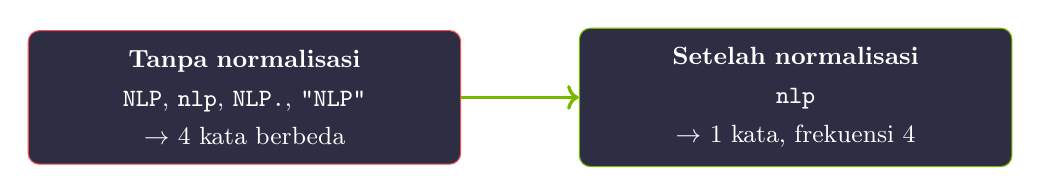
\begin{tikzpicture}[font=\small]
    \node[draw=nvred, fill=nvcard, rounded corners=4pt, text=nvwhite,
          text width=5cm, align=center, inner sep=7pt] (a) at (0,0)
          {\textbf{Tanpa normalisasi}\\[3pt]
           \texttt{NLP}, \texttt{nlp}, \texttt{NLP.}, \texttt{"NLP"}\\[3pt]
           $\to$ 4 kata berbeda};
    \node[draw=nvgreen, fill=nvcard, rounded corners=4pt, text=nvwhite,
          text width=5cm, align=center, inner sep=7pt] (b) at (7,0)
          {\textbf{Setelah normalisasi}\\[3pt]
           \texttt{nlp}\\[3pt]
           $\to$ 1 kata, frekuensi 4};
    \draw[->,very thick,color=nvgreen] (a) -- (b);
  \end{tikzpicture}%
  }
  \end{center}
  \vspace{0.6em}
  \begin{center}
    {\color{nvlightgreen}\small Setiap variasi ejaan yang tidak disatukan menjadi satu dimensi
    fitur tambahan yang harus dipelajari model dari nol.}
  \end{center}
\end{frame}

\begin{frame}{Stopword: Kata yang Tidak Membedakan}
  \begin{columns}[T]
    \begin{column}{0.52\textwidth}
      \begin{itemize}
        \footnotesize
        \item Kata yang muncul di hampir semua dokumen
        \item Indonesia: \texttt{yang, di, dari, dan, adalah}
        \item Inggris: \texttt{the, is, are, of}
        \item Membuangnya memperkecil dimensi fitur
        \item[\textcolor{nvgreen}{\checkmark}] \texttt{nlp-id}: \texttt{StopWord().get\_stopword()}
        \item[\textcolor{nvgreen}{\checkmark}] NLTK: \texttt{stopwords.words('english')}
      \end{itemize}
    \end{column}
    \begin{column}{0.44\textwidth}
      \begin{center}
      \resizebox{\linewidth}{!}{%
      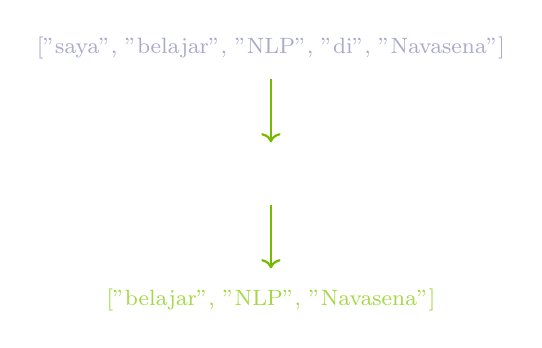
\begin{tikzpicture}[font=\footnotesize]
        \node[text=nvgray] at (0,2.6) {["saya", "belajar", "NLP", "di", "Navasena"]};
        \draw[->,thick,color=nvgreen] (0,2.2) -- (0,1.4);
        \node[text=nvwhite] at (0,1.0) {buang stopword};
        \draw[->,thick,color=nvgreen] (0,0.6) -- (0,-0.2);
        \node[text=nvlightgreen] at (0,-0.6) {["belajar", "NLP", "Navasena"]};
      \end{tikzpicture}%
      }
      \end{center}
    \end{column}
  \end{columns}
  \vspace{0.5em}
  \jebakan{Stopword bukan daftar universal. Untuk analisis negasi, membuang
  \texttt{tidak} justru menghapus informasi yang paling menentukan.}
\end{frame}

\begin{frame}{Lemmatisasi vs Stemming}
  \begin{columns}[T]
    \begin{column}{0.48\textwidth}
      \textcolor{nvorange}{\textbf{Stemming}}
      \begin{itemize}
        \footnotesize
        \item Memotong imbuhan secara mekanis
        \item Cepat, tidak butuh kamus
        \item Hasilnya boleh bukan kata: \texttt{mempelajari $\to$ pelajar}
      \end{itemize}
    \end{column}
    \begin{column}{0.48\textwidth}
      \textcolor{nvgreen}{\textbf{Lemmatisasi}}
      \begin{itemize}
        \footnotesize
        \item Berbasis kamus dan aturan morfologi
        \item Lebih lambat, lebih akurat
        \item Hasilnya selalu kata: \texttt{mempelajari $\to$ ajar}
      \end{itemize}
    \end{column}
  \end{columns}
  \vspace{0.8em}
  \begin{beamercolorbox}[rounded=true,shadow=false,sep=6pt]{block body}
    \small\color{white}
    \texttt{nlp-id} menyediakan \texttt{Lemmatizer().lemmatize()}.
    \textbf{Sastrawi} masih sering dikutip untuk stemming Indonesia, tetapi
    rilis terakhirnya tahun 2016 --- perlakukan sebagai referensi historis.
  \end{beamercolorbox}
\end{frame}

\begin{frame}{POS Tagging: Menandai Kelas Kata}
  \begin{columns}[T]
    \begin{column}{0.48\textwidth}
      \begin{center}
      \resizebox{\linewidth}{!}{%
      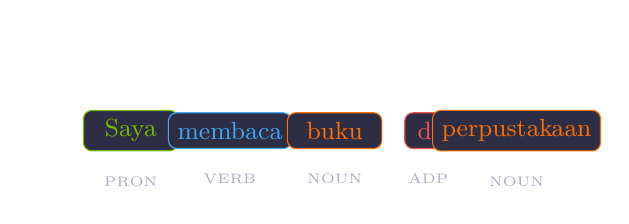
\begin{tikzpicture}[scale=0.7]
        \node[text=nvwhite, font=\small\bfseries] at (0,3) {"Saya membaca buku di perpustakaan."};
        \node[draw=nvgreen, fill=nvcard, rounded corners=3pt,
              text=nvgreen, font=\small, minimum width=1.2cm] (w1) at (-3,1.5) {Saya};
        \node[draw=nvblue, fill=nvcard, rounded corners=3pt,
              text=nvblue, font=\small, minimum width=1.5cm] (w2) at (-1.2,1.5) {membaca};
        \node[draw=nvorange, fill=nvcard, rounded corners=3pt,
              text=nvorange, font=\small, minimum width=1.2cm] (w3) at (0.7,1.5) {buku};
        \node[draw=nvred, fill=nvcard, rounded corners=3pt,
              text=nvred, font=\small, minimum width=0.6cm] (w4) at (2.4,1.5) {di};
        \node[draw=nvorange, fill=nvcard, rounded corners=3pt,
              text=nvorange, font=\small, minimum width=2cm] (w5) at (4,1.5) {perpustakaan};
        \node[text=nvgray, font=\tiny, below=0.2cm of w1] {PRON};
        \node[text=nvgray, font=\tiny, below=0.2cm of w2] {VERB};
        \node[text=nvgray, font=\tiny, below=0.2cm of w3] {NOUN};
        \node[text=nvgray, font=\tiny, below=0.2cm of w4] {ADP};
        \node[text=nvgray, font=\tiny, below=0.2cm of w5] {NOUN};
      \end{tikzpicture}%
      }
      \end{center}
    \end{column}
    \begin{column}{0.48\textwidth}
      \begin{itemize}
        \footnotesize
        \item \textbf{POS} = \emph{part of speech}, kelas kata
        \item Dipakai untuk menyaring kandidat topik (ambil kata benda saja)
        \item Juga untuk penerjemahan mesin dan ekstraksi informasi
      \end{itemize}
    \end{column}
  \end{columns}
  \vspace{0.3em}
  {\color{nvgray}\scriptsize Catatan: label di slide memakai tagset UD (ilustratif); \texttt{nlp-id} memakai NNP/VB/NN/IN.}
\end{frame}

\begin{frame}{Tokenisasi Frasa: Entitas Multi-kata}
  \begin{center}
  \resizebox{0.92\linewidth}{!}{%
  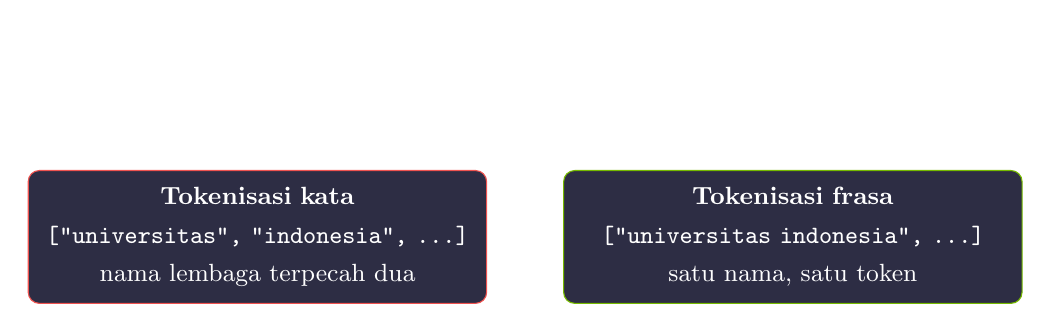
\begin{tikzpicture}[font=\small]
    \node[text=nvwhite] at (0,2.4) {"Universitas Indonesia adalah kampus terbaik di Jakarta."};
    \node[draw=nvred, fill=nvcard, rounded corners=4pt, text=nvwhite,
          text width=5.4cm, align=center, inner sep=6pt] (a) at (-3.4,0)
          {\textbf{Tokenisasi kata}\\[3pt]
           \texttt{["universitas", "indonesia", ...]}\\[3pt]
           nama lembaga terpecah dua};
    \node[draw=nvgreen, fill=nvcard, rounded corners=4pt, text=nvwhite,
          text width=5.4cm, align=center, inner sep=6pt] (b) at (3.4,0)
          {\textbf{Tokenisasi frasa}\\[3pt]
           \texttt{["universitas indonesia", ...]}\\[3pt]
           satu nama, satu token};
  \end{tikzpicture}%
  }
  \end{center}
  \vspace{0.6em}
  \begin{itemize}
    \footnotesize
    \item \texttt{PhraseTokenizer} mengelompokkan frasa nomina jadi satu token
    \item Berguna sebelum analisis frekuensi: "kecerdasan buatan" tidak tercerai
    \item Bukan NER --- ia menemukan frasa, tetapi tidak memberi label jenis entitas
  \end{itemize}
\end{frame}

\begin{frame}{Ringkasan Act 2}
  \begin{center}
  \renewcommand{\arraystretch}{1.25}
  {\footnotesize
  \begin{tabular}{@{}p{0.30\linewidth}p{0.62\linewidth}@{}}
    \toprule
    \rowcolor{nvcard!50}
    \textbf{Langkah} & \textbf{Yang dilakukan} \\
    \midrule
    Normalisasi & Huruf kecil, buang angka dan tanda baca, rapikan spasi \\
    Tokenisasi & Pecah teks jadi kata (atau frasa) \\
    Stopword & Buang kata yang tidak membedakan dokumen \\
    Lemmatisasi & Kembalikan kata ke bentuk dasar berbasis kamus \\
    POS tagging & Tandai kelas kata untuk penyaringan lanjutan \\
    \bottomrule
  \end{tabular}%
  }
  \end{center}
  \vspace{0.8em}
  \begin{center}
    {\color{nvlightgreen}\small Keluaran Act 2: daftar token bersih --- bahan baku untuk semua act berikutnya.}
  \end{center}
\end{frame}

% ============================================================
% ACT 3 — MENGANALISIS TEKS
% ============================================================
\acttitle{3}{Menganalisis Teks}{Apa yang dibicarakan dokumen ini, dan siapa yang disebut?}

\begin{frame}{Frekuensi Kata: Menebak Topik}
  \begin{center}
    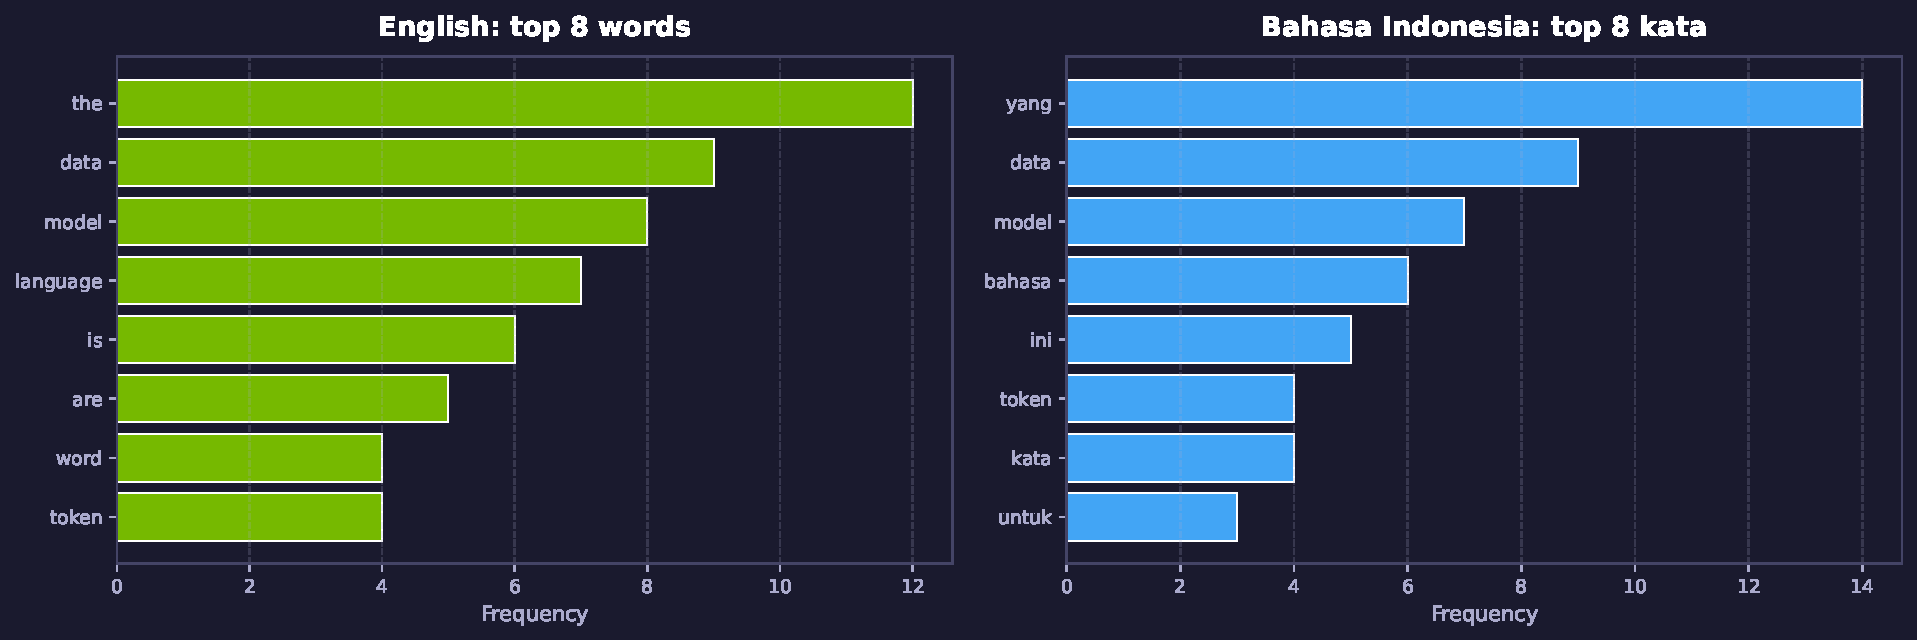
\includegraphics[width=0.95\textwidth]{figures/word_frequency.pdf}
  \end{center}
  \vspace{0.2em}
  {\small\centering\textcolor{nvlightgreen}{Stopword Inggris: \texttt{the, is, are} \quad$\cdot$\quad Stopword Indonesia: \texttt{yang, di, dari, dan}}}
\end{frame}

\begin{frame}
  \intuisi{Frekuensi tanpa pembersihan tidak memberi tahu apa pun}
  \vspace{0.5em}
  \begin{columns}[T]
    \begin{column}{0.48\textwidth}
      \textcolor{nvred}{\textbf{Teks mentah, top-5}}
      \begin{enumerate}
        \footnotesize
        \item \texttt{yang}
        \item \texttt{di}
        \item \texttt{dan}
        \item \texttt{adalah}
        \item \texttt{untuk}
      \end{enumerate}
      \vspace{0.3em}
      {\footnotesize\color{nvgray}Daftar ini sama untuk dokumen apa pun.}
    \end{column}
    \begin{column}{0.48\textwidth}
      \textcolor{nvgreen}{\textbf{Setelah dibersihkan, top-5}}
      \begin{enumerate}
        \footnotesize
        \item \texttt{nlp}
        \item \texttt{kembang}
        \item \texttt{indonesia}
        \item \texttt{model}
        \item \texttt{bahasa}
      \end{enumerate}
      \vspace{0.3em}
      {\footnotesize\color{nvgray}Baru di sini topiknya terbaca.}
    \end{column}
  \end{columns}
  \vspace{0.7em}
  \begin{center}
    {\color{nvlightgreen}\small Pembersihan bukan pekerjaan rumah tangga --- ia yang menentukan
    apakah hasil analisis punya isi.}
  \end{center}
\end{frame}

\begin{frame}{Word Cloud: Cantik, tapi Hati-hati}
  \begin{columns}[T]
    \begin{column}{0.5\textwidth}
      \textcolor{nvgreen}{\textbf{Kelebihan}}
      \begin{itemize}
        \footnotesize
        \item Sekali lihat langsung menangkap tema
        \item Bagus untuk presentasi dan laporan awam
      \end{itemize}
      \vspace{0.4em}
      \textcolor{nvred}{\textbf{Kekurangan}}
      \begin{itemize}
        \footnotesize
        \item Mata sulit membandingkan luas huruf
        \item Tata letaknya acak, bukan informasi
        \item Tidak bisa dibaca sebagai angka
      \end{itemize}
    \end{column}
    \begin{column}{0.46\textwidth}
      \begin{center}
      \resizebox{\linewidth}{!}{%
      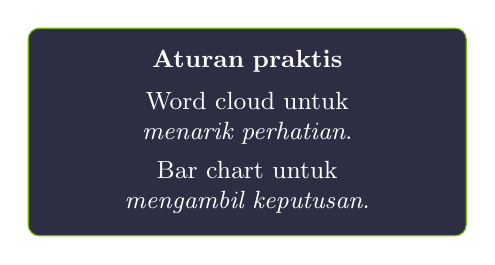
\begin{tikzpicture}[font=\small]
        \node[draw=nvgreen, fill=nvcard, rounded corners=4pt, text=nvwhite,
              text width=5cm, align=center, inner sep=8pt]
          {\textbf{Aturan praktis}\\[4pt]
           Word cloud untuk \emph{menarik perhatian}.\\[3pt]
           Bar chart untuk \emph{mengambil keputusan}.};
      \end{tikzpicture}%
      }
      \end{center}
    \end{column}
  \end{columns}
\end{frame}

\begin{frame}{Named Entity Recognition (NER)}
  \begin{center}
  \resizebox{\linewidth}{!}{%
  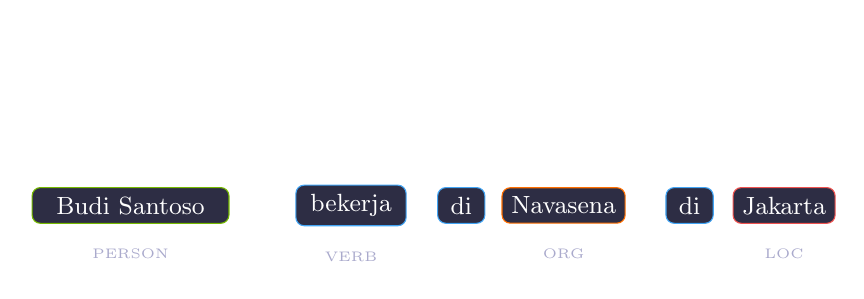
\begin{tikzpicture}
    \node[text=nvwhite, font=\small] at (0,2.5) {"Budi Santoso bekerja di Navasena di Jakarta sejak 2024."};
    \node[draw=nvgreen, fill=nvcard, rounded corners=3pt,
          text=nvwhite, font=\small, minimum width=2.5cm] (p) at (-3,0.5) {Budi Santoso};
    \node[draw=nvblue, fill=nvcard, rounded corners=3pt,
          text=nvwhite, font=\small, minimum width=1.4cm] (v) at (-0.2,0.5) {bekerja};
    \node[draw=nvblue, fill=nvcard, rounded corners=3pt,
          text=nvwhite, font=\small, minimum width=0.6cm] (v2) at (1.2,0.5) {di};
    \node[draw=nvorange, fill=nvcard, rounded corners=3pt,
          text=nvwhite, font=\small, minimum width=1.4cm] (o) at (2.5,0.5) {Navasena};
    \node[draw=nvblue, fill=nvcard, rounded corners=3pt,
          text=nvwhite, font=\small, minimum width=0.6cm] (v3) at (4.1,0.5) {di};
    \node[draw=nvred, fill=nvcard, rounded corners=3pt,
          text=nvwhite, font=\small, minimum width=1.2cm] (l) at (5.3,0.5) {Jakarta};
    \node[text=nvgray, font=\tiny, below=0.2cm of p] {PERSON};
    \node[text=nvgray, font=\tiny, below=0.2cm of v] {VERB};
    \node[text=nvgray, font=\tiny, below=0.2cm of o] {ORG};
    \node[text=nvgray, font=\tiny, below=0.2cm of l] {LOC};
  \end{tikzpicture}%
  }
  \end{center}
  \vspace{0.3em}
  \begin{itemize}
    \footnotesize
    \item[\textcolor{nvgreen}{\checkmark}] \textbf{PERSON} (orang) \quad $\cdot$ \quad
          \textbf{ORG} (organisasi) \quad $\cdot$ \quad
          \textbf{LOC} (lokasi) \quad $\cdot$ \quad \textbf{DATE} (tanggal)
  \end{itemize}
  {\color{nvgray}\scriptsize spaCy melabeli kota/negara sebagai GPE (bukan LOC).}
\end{frame}

\begin{frame}{NER untuk Apa? Tiga Kasus Nyata}
  \begin{columns}[T]
    \begin{column}{0.32\textwidth}
      \begin{center}
      \nvbox{Kontrak}{\footnotesize Tarik nama pihak, nilai, dan tanggal berlaku dari ratusan dokumen PDF.}
      \end{center}
    \end{column}
    \begin{column}{0.32\textwidth}
      \begin{center}
      \nvbox{Berita}{\footnotesize Pantau setiap penyebutan nama perusahaan di media, lalu gabungkan dengan sentimennya.}
      \end{center}
    \end{column}
    \begin{column}{0.32\textwidth}
      \begin{center}
      \nvbox{Layanan}{\footnotesize Isi otomatis formulir tiket dari keluhan pelanggan berbentuk teks bebas.}
      \end{center}
    \end{column}
  \end{columns}
  \vspace{0.9em}
  \begin{center}
    {\color{nvlightgreen}\small Pola yang sama: teks bebas masuk, data terstruktur keluar.}
  \end{center}
\end{frame}

\begin{frame}{NER Bahasa Indonesia: Tiga Jalur}
  \begin{center}
  \renewcommand{\arraystretch}{1.3}
  {\footnotesize
  \begin{tabular}{@{}p{0.30\linewidth}p{0.30\linewidth}p{0.32\linewidth}@{}}
    \toprule
    \rowcolor{nvcard!50}
    \textbf{Jalur} & \textbf{Kelebihan} & \textbf{Batasan} \\
    \midrule
    spaCy \texttt{xx\_ent\_wiki\_sm} & Multibahasa, ringan & Akurasi sedang \\
    Model NER IndoBERT di Hugging Face & Akurasi terbaik untuk Indonesia & Unduhan besar, butuh GPU agar cepat \\
    \texttt{PhraseTokenizer} (\texttt{nlp-id}) & Tanpa model, sangat cepat & Menemukan frasa, tidak memberi label \\
    \bottomrule
  \end{tabular}%
  }
  \end{center}
  \vspace{0.7em}
  \begin{center}
    {\color{nvgray}\small spaCy belum menyediakan pipeline khusus bahasa Indonesia.}
  \end{center}
\end{frame}

\begin{frame}{Ringkasan Act 3}
  \begin{itemize}
    \item[\textcolor{nvgreen}{\checkmark}] \textbf{Frekuensi kata} menebak topik --- selalu setelah pembersihan
    \item[\textcolor{nvgreen}{\checkmark}] \textbf{Word cloud} untuk menarik perhatian, \textbf{bar chart} untuk keputusan
    \item[\textcolor{nvgreen}{\checkmark}] \textbf{NER} mengubah teks bebas menjadi data terstruktur
    \item[\textcolor{nvgreen}{\checkmark}] Untuk Indonesia, NER berkualitas berarti memakai model transformer
  \end{itemize}
  \vspace{0.9em}
  \begin{center}
    {\color{nvlightgreen}\small Act 3 masih \emph{menggambarkan} teks. Act 4 mulai \emph{menilai}-nya.}
  \end{center}
\end{frame}

% ============================================================
% ACT 4 — MENILAI TEKS
% ============================================================
\acttitle{4}{Menilai Teks}{Sentimen dan klasifikasi --- dan satu kesalahan yang sering lolos}

\begin{frame}{Analisis Sentimen: Dua Generasi}
  \begin{columns}[T]
    \begin{column}{0.48\textwidth}
      \textcolor{nvblue}{\textbf{Generasi 1 --- leksikon}}
      \begin{itemize}
        \footnotesize
        \item Kamus kata beserta skor sentimennya
        \item Skor kata dijumlahkan
        \item Cepat, transparan, tanpa GPU
        \item Contoh: \texttt{TextBlob}
      \end{itemize}
    \end{column}
    \begin{column}{0.48\textwidth}
      \textcolor{nvorange}{\textbf{Generasi 2 --- transformer}}
      \begin{itemize}
        \footnotesize
        \item Model dilatih dari teks nyata berlabel
        \item Membaca susunan kalimat, bukan menjumlah
        \item Butuh unduhan ratusan MB
        \item Contoh: \texttt{IndoBERT}
      \end{itemize}
    \end{column}
  \end{columns}
  \vspace{0.7em}
  \begin{beamercolorbox}[rounded=true,shadow=false,sep=4pt]{block body}
    \small\color{white}
    \textbf{TextBlob}: \texttt{polarity} $\in [-1{,}0;\ 1{,}0]$ \quad $\cdot$ \quad
    \texttt{subjectivity} $\in [0{,}0;\ 1{,}0]$
  \end{beamercolorbox}
\end{frame}

\begin{frame}{Skala Polaritas}
  \begin{center}
  \resizebox{0.85\linewidth}{!}{%
  
\begin{tikzpicture}
    \draw[->,thick,color=nvwhite] (-3,0) -- (3,0);
    \node[color=nvred, font=\small\bfseries, above] at (-2.7,0.1) {Negatif};
    \node[color=nvwhite, font=\small] at (-1.8,0.4) {-1,0};
    \node[color=nvgray, font=\small] at (0,0.4) {0,0};
    \node[color=nvwhite, font=\small] at (1.8,0.4) {+1,0};
    \node[color=nvgreen, font=\small\bfseries, above] at (2.7,0.1) {Positif};
    \fill[color=nvred, opacity=0.6] (-2.5,-0.1) circle (0.18);
    \fill[color=nvorange, opacity=0.6] (-0.5,-0.1) circle (0.18);
    \fill[color=nvgreen, opacity=0.6] (2.0,-0.1) circle (0.18);
    \node[color=nvred, font=\tiny, below=0.1cm] at (-2.5,-0.3) {"jelek"};
    \node[color=nvorange, font=\tiny, below=0.1cm] at (-0.5,-0.3) {"biasa"};
    \node[color=nvgreen, font=\tiny, below=0.1cm] at (2.0,-0.3) {"hebat"};
  \end{tikzpicture}%
  }
  \end{center}
  \vspace{0.8em}
  \jebakan{Skor \texttt{0,0} punya dua arti yang sangat berbeda: kalimat benar-benar
  netral, atau tidak ada satu pun katanya yang ada di kamus. Leksikon tidak
  membedakan keduanya.}
\end{frame}

\begin{frame}{Batas Leksikon: Negasi Jauh dan Sarkasme}
  \begin{center}
  \renewcommand{\arraystretch}{1.35}
  {\footnotesize
  \begin{tabular}{@{}p{0.54\linewidth}p{0.14\linewidth}p{0.24\linewidth}@{}}
    \toprule
    \rowcolor{nvcard!50}
    \textbf{Kalimat} & \textbf{TextBlob} & \textbf{Maksudnya} \\
    \midrule
    \texttt{The plot was not good.} & \textcolor{nvgreen}{$-0{,}35$} & negatif \checkmark \\
    \texttt{I would not call this a great movie.} & \textcolor{nvred}{$+0{,}80$} & negatif \ding{55} \\
    \texttt{Nobody would say this restaurant is bad.} & \textcolor{nvred}{$-0{,}70$} & positif \ding{55} \\
    \bottomrule
  \end{tabular}%
  }
  \end{center}
  \vspace{0.5em}
  \begin{itemize}
    \footnotesize
    \item Baris pertama benar: \texttt{not} membalik skor kata \textbf{tepat sesudahnya}
    \item Baris kedua meleset karena \texttt{not} berjarak tiga kata dari \texttt{great}
    \item Sarkasme meleset sepenuhnya --- isyaratnya ada di konteks, bukan di kata
  \end{itemize}
\end{frame}

\begin{frame}{Batas Leksikon: Bahasa}
  \begin{center}
  \resizebox{0.88\linewidth}{!}{%
  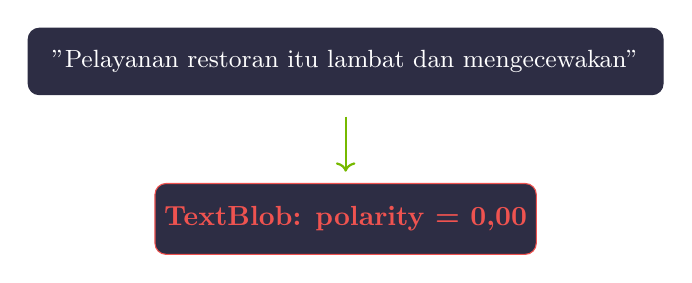
\begin{tikzpicture}[font=\small]
    \node[draw=nvcard, fill=nvcard, rounded corners=4pt, text=nvwhite,
          text width=7.5cm, align=center, inner sep=8pt] (in) at (0,1.4)
          {"Pelayanan restoran itu lambat dan mengecewakan"};
    \draw[->,thick,color=nvgreen] (0,0.7) -- (0,0.0);
    \node[draw=nvred, fill=nvcard, rounded corners=4pt, text=nvred,
          font=\bfseries, minimum width=4cm, minimum height=0.9cm] (out) at (0,-0.6)
          {TextBlob: polarity = 0,00};
  \end{tikzpicture}%
  }
  \end{center}
  \vspace{0.7em}
  \jebakan{Nol di sini bukan "netral". Kamus TextBlob hanya berbahasa Inggris,
  jadi tidak ada satu pun kata Indonesia yang dikenali. Nol berarti "tidak tahu",
  dan model tidak akan memberi tahu kamu bedanya.}
\end{frame}

\begin{frame}[fragile]{Sentimen Indonesia dengan IndoBERT}
  \begin{lstlisting}[language=Python]
sentimen = pipeline("sentiment-analysis",
    model="w11wo/indonesian-roberta-base-sentiment-classifier")
sentimen("Gw suka bgt sama teknologi NLP nih")
# [{'label': 'positive', 'score': 0.99}]
  \end{lstlisting}
  \vspace{0.2em}
  \begin{itemize}
    \footnotesize
    \item Transformer yang di-\emph{fine-tune} untuk bahasa Indonesia --- tahan bahasa gaul
    \item Pola transfer learning yang sama dengan ResNet di Modul 02
    \item Mengenali tiga kelas: positif, negatif, dan netral
    \item Ekosistem: IndoBERT, IndoNLU, IndoLEM, NusaBERT (Hugging Face Hub)
  \end{itemize}
\end{frame}

\begin{frame}
  \intuisi{Kenapa transformer tahan bahasa gaul}
  \vspace{0.4em}
  \begin{columns}[T]
    \begin{column}{0.48\textwidth}
      \textcolor{nvred}{\textbf{Leksikon}}
      \begin{itemize}
        \footnotesize
        \item Kamusnya disusun manusia dari teks baku
        \item \texttt{gw}, \texttt{bgt}, \texttt{anjir} tidak ada di dalamnya
        \item Menambah kata baru berarti menyunting kamus
      \end{itemize}
    \end{column}
    \begin{column}{0.48\textwidth}
      \textcolor{nvgreen}{\textbf{Transformer}}
      \begin{itemize}
        \footnotesize
        \item Dilatih dari teks nyata: Twitter, ulasan, forum
        \item Bahasa gaul ikut terlatih karena memang ada di data
        \item Subword membuat kata tak dikenal tetap terwakili
      \end{itemize}
    \end{column}
  \end{columns}
  \vspace{0.8em}
  \begin{center}
    {\color{nvlightgreen}\small Bedanya bukan kecerdasan model, melainkan dari mana pengetahuannya berasal:
    kamus yang disusun, atau data yang dikumpulkan.}
  \end{center}
\end{frame}

\begin{frame}{Leksikon atau Transformer?}
  \kapan{
    \footnotesize
    \item Jutaan dokumen, butuh penyaringan kasar
    \item Tanpa GPU, harus jalan di CPU biasa
    \item Skor harus bisa dijelaskan per kata
    \item Teks Inggris baku
  }{
    \footnotesize
    \item Teks Indonesia atau bahasa informal
    \item Negasi dan sarkasme penting
    \item Butuh kelas netral yang benar
    \item Akurasi lebih penting daripada kecepatan
  }
  \vspace{0.9em}
  \begin{center}
    {\color{nvlightgreen}\small Keduanya sering dipakai bersama: leksikon menyaring, transformer memutuskan.}
  \end{center}
\end{frame}

\begin{frame}{Klasifikasi Teks: Bag-of-Words}
  \begin{center}
  \resizebox{0.92\linewidth}{!}{%
  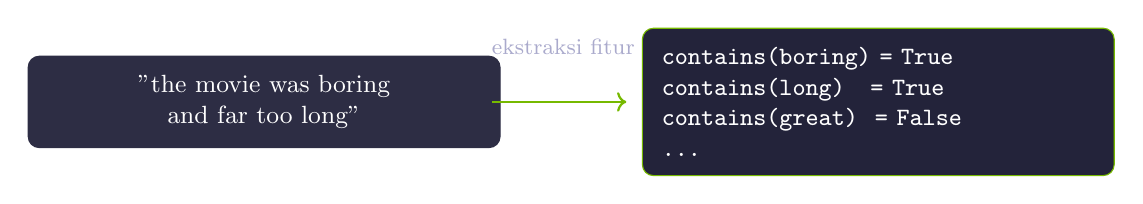
\begin{tikzpicture}[font=\small]
    \node[draw=nvcard, fill=nvcard, rounded corners=4pt, text=nvwhite,
          text width=5.5cm, align=center, inner sep=7pt] (doc) at (-4,0)
          {"the movie was boring\\and far too long"};
    \draw[->,thick,color=nvgreen] (-1.1,0) -- (0.6,0);
    \node[draw=nvgreen, fill=nvdarkcard, rounded corners=4pt, text=nvwhite,
          text width=5.5cm, align=left, inner sep=7pt] (vec) at (3.8,0)
          {\texttt{contains(boring) = True}\\
           \texttt{contains(long)\ \ \ = True}\\
           \texttt{contains(great)\ \ = False}\\
           \texttt{...}};
    \node[text=nvgray, font=\footnotesize] at (-0.2,0.7) {ekstraksi fitur};
  \end{tikzpicture}%
  }
  \end{center}
  \vspace{0.7em}
  \begin{itemize}
    \footnotesize
    \item Urutan kata dibuang total --- yang dihitung hanya kehadiran
    \item Setiap dokumen jadi vektor \texttt{True}/\texttt{False} sepanjang kosakata fitur
    \item Sederhana, tetapi inilah bentuk paling awal dari "teks sebagai vektor"
  \end{itemize}
\end{frame}

\begin{frame}{Naive Bayes: Kenapa Masih Diajarkan}
  \begin{columns}[T]
    \begin{column}{0.5\textwidth}
      \begin{itemize}
        \footnotesize
        \item Menghitung P(kelas $\mid$ fitur) lewat Teorema Bayes
        \item "Naive" karena menganggap setiap kata muncul saling bebas ---
              asumsi yang salah, tetapi bekerja baik untuk teks
        \item Latihnya sangat cepat, bahkan di data besar
        \item Keputusannya \textbf{bisa dibaca manusia}
      \end{itemize}
    \end{column}
    \begin{column}{0.46\textwidth}
      \begin{center}
      \resizebox{\linewidth}{!}{%
      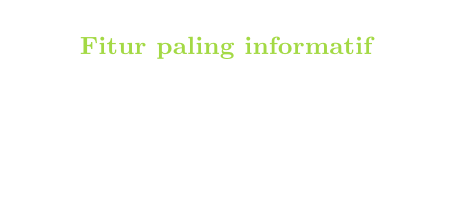
\begin{tikzpicture}[font=\footnotesize]
        \node[text=nvlightgreen, font=\small\bfseries] at (0,1.6) {Fitur paling informatif};
        \node[text=nvwhite, align=left] at (0,0.4)
          {\texttt{outstanding}\quad pos : neg = 11,8 : 1,0\\[2pt]
           \texttt{wonderfully}\quad pos : neg = \ 6,5 : 1,0\\[2pt]
           \texttt{poorly}\ \ \ \ \ \quad neg : pos = \ 5,7 : 1,0};
      \end{tikzpicture}%
      }
      \end{center}
      \vspace{0.2em}
      {\footnotesize\color{nvgray}Dibaca: kata itu 11,8x lebih sering muncul di ulasan positif.}
    \end{column}
  \end{columns}
\end{frame}

\begin{frame}
  \intuisi{Kebocoran data: kesalahan yang tidak menimbulkan error}
  \vspace{0.3em}
  \begin{center}
  \resizebox{0.95\linewidth}{!}{%
  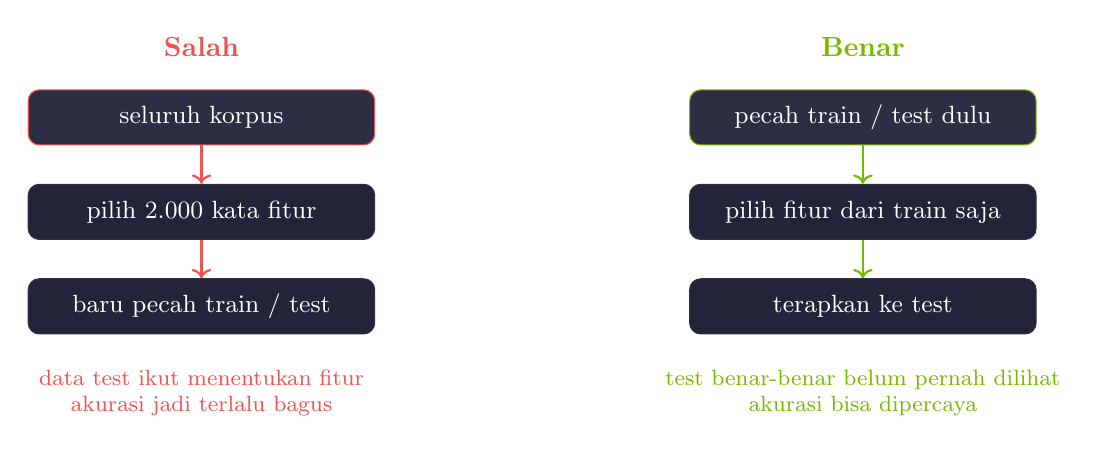
\begin{tikzpicture}[font=\small]
    % SALAH
    \node[text=nvred, font=\bfseries] at (-4.2,2.6) {Salah};
    \node[draw=nvred, fill=nvcard, rounded corners=4pt, text=nvwhite,
          minimum width=4.4cm, minimum height=0.7cm] (a1) at (-4.2,1.7) {seluruh korpus};
    \node[draw=nvcard, fill=nvdarkcard, rounded corners=4pt, text=nvwhite,
          minimum width=4.4cm, minimum height=0.7cm] (a2) at (-4.2,0.5) {pilih 2.000 kata fitur};
    \node[draw=nvcard, fill=nvdarkcard, rounded corners=4pt, text=nvwhite,
          minimum width=4.4cm, minimum height=0.7cm] (a3) at (-4.2,-0.7) {baru pecah train / test};
    \draw[->,thick,color=nvred] (a1) -- (a2);
    \draw[->,thick,color=nvred] (a2) -- (a3);
    \node[text=nvred, font=\footnotesize, align=center] at (-4.2,-1.8)
      {data test ikut menentukan fitur\\akurasi jadi terlalu bagus};
    % BENAR
    \node[text=nvgreen, font=\bfseries] at (4.2,2.6) {Benar};
    \node[draw=nvgreen, fill=nvcard, rounded corners=4pt, text=nvwhite,
          minimum width=4.4cm, minimum height=0.7cm] (b1) at (4.2,1.7) {pecah train / test dulu};
    \node[draw=nvcard, fill=nvdarkcard, rounded corners=4pt, text=nvwhite,
          minimum width=4.4cm, minimum height=0.7cm] (b2) at (4.2,0.5) {pilih fitur dari train saja};
    \node[draw=nvcard, fill=nvdarkcard, rounded corners=4pt, text=nvwhite,
          minimum width=4.4cm, minimum height=0.7cm] (b3) at (4.2,-0.7) {terapkan ke test};
    \draw[->,thick,color=nvgreen] (b1) -- (b2);
    \draw[->,thick,color=nvgreen] (b2) -- (b3);
    \node[text=nvgreen, font=\footnotesize, align=center] at (4.2,-1.8)
      {test benar-benar belum pernah dilihat\\akurasi bisa dipercaya};
  \end{tikzpicture}%
  }
  \end{center}
\end{frame}

\begin{frame}{Aturan yang Sama Berlaku untuk Semuanya}
  \begin{center}
  \renewcommand{\arraystretch}{1.25}
  {\footnotesize
  \begin{tabular}{@{}p{0.32\linewidth}p{0.60\linewidth}@{}}
    \toprule
    \rowcolor{nvcard!50}
    \textbf{Langkah} & \textbf{Yang dipelajari dari data} \\
    \midrule
    Seleksi fitur & Kata mana yang dipakai sebagai kolom \\
    \texttt{TfidfVectorizer} & Kosakata dan bobot IDF \\
    \texttt{StandardScaler} & Rata-rata dan simpangan baku \\
    Imputasi nilai kosong & Median atau modus pengisi \\
    \bottomrule
  \end{tabular}%
  }
  \end{center}
  \vspace{0.8em}
  \begin{center}
    {\color{nvlightgreen}\small Semuanya di-\texttt{fit} pada train, lalu diterapkan ke test.
    Melanggarnya tidak memunculkan error --- hanya angka yang menyenangkan dan salah.}
  \end{center}
\end{frame}

\begin{frame}{Baseline: Angka Pembanding yang Wajib}
  \begin{center}
  \resizebox{0.85\linewidth}{!}{%
  
\begin{tikzpicture}[font=\small]
    \node[draw=nvcard, fill=nvcard, rounded corners=4pt, text=nvwhite,
          text width=5.6cm, align=center, inner sep=8pt] (a) at (-3.4,0)
          {\textbf{Akurasi model}\\[4pt]{\Large\color{nvgreen}78,0\%}};
    \node[draw=nvcard, fill=nvcard, rounded corners=4pt, text=nvwhite,
          text width=5.6cm, align=center, inner sep=8pt] (b) at (3.4,0)
          {\textbf{Baseline kelas mayoritas}\\[4pt]{\Large\color{nvorange}54,8\%}};
  \end{tikzpicture}%
  }
  \end{center}
  \vspace{0.8em}
  \begin{itemize}
    \footnotesize
    \item \textbf{Baseline kelas mayoritas} = akurasi kalau selalu menebak kelas terbanyak
    \item \texttt{movie\_reviews} seimbang 1.000 lawan 1.000, jadi baseline dekat 50\%
    \item Kalau 95\% data satu kelas, akurasi 94\% berarti model lebih buruk daripada menebak
  \end{itemize}
  \vspace{0.4em}
  \jebakan{Akurasi tanpa baseline adalah angka tanpa arti. Selalu laporkan keduanya.}
\end{frame}

\begin{frame}{Ringkasan Act 4}
  \begin{itemize}
    \item[\textcolor{nvgreen}{\checkmark}] Sentimen leksikon cepat dan transparan, tetapi buta terhadap negasi dan bahasa non-Inggris
    \item[\textcolor{nvgreen}{\checkmark}] Transformer Indonesia (IndoBERT) tahan bahasa gaul dan mengenali kelas netral
    \item[\textcolor{nvgreen}{\checkmark}] Bag-of-words membuang urutan kata --- \texttt{"not good"} dan \texttt{"good"} bersinyal sama
    \item[\textcolor{nvgreen}{\checkmark}] Apa pun yang belajar dari data harus di-\texttt{fit} pada train saja
    \item[\textcolor{nvgreen}{\checkmark}] Akurasi selalu dilaporkan bersama baseline kelas mayoritas
  \end{itemize}
  \vspace{0.7em}
  \begin{center}
    {\color{nvlightgreen}\small Masalah yang tersisa: hitungan kata tidak tahu bahwa "suka" dan "gemar" itu sama.
    Act 5 menyelesaikannya.}
  \end{center}
\end{frame}

% ============================================================
% ACT 5 — DARI KATA KE MAKNA
% ============================================================
\acttitle{5}{Dari Kata ke Makna}{Jembatan menuju LLM (Modul 04) dan RAG (Modul 05)}

\begin{frame}{Tiga Anak Tangga Representasi Teks}
  \begin{center}
  \resizebox{0.95\linewidth}{!}{%
  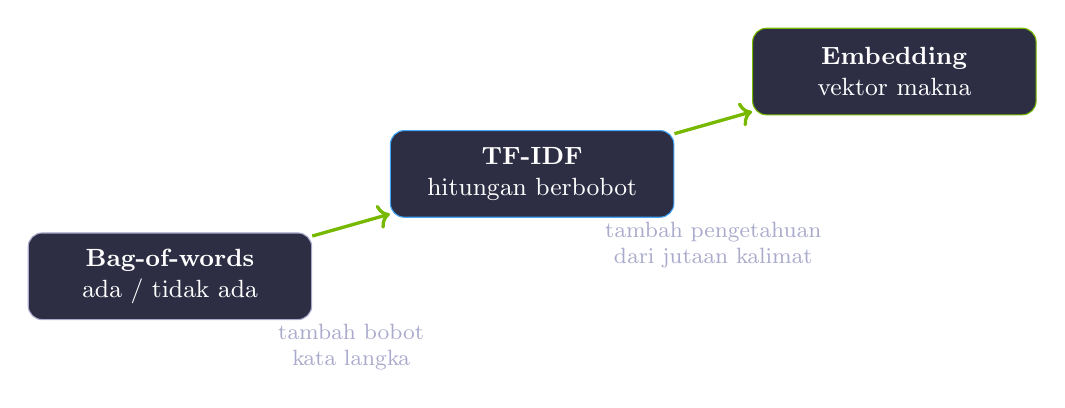
\begin{tikzpicture}[font=\small]
    \node[draw=nvgray, fill=nvcard, rounded corners=5pt, text=nvwhite,
          minimum width=3.6cm, minimum height=1.1cm, align=center] (a) at (0,0)
          {\textbf{Bag-of-words}\\ada / tidak ada};
    \node[draw=nvblue, fill=nvcard, rounded corners=5pt, text=nvwhite,
          minimum width=3.6cm, minimum height=1.1cm, align=center] (b) at (4.6,1.3)
          {\textbf{TF-IDF}\\hitungan berbobot};
    \node[draw=nvgreen, fill=nvcard, rounded corners=5pt, text=nvwhite,
          minimum width=3.6cm, minimum height=1.1cm, align=center] (c) at (9.2,2.6)
          {\textbf{Embedding}\\vektor makna};
    \draw[->,very thick,color=nvgreen] (a) -- (b);
    \draw[->,very thick,color=nvgreen] (b) -- (c);
    \node[text=nvgray, font=\footnotesize, align=center] at (2.3,-0.9) {tambah bobot\\kata langka};
    \node[text=nvgray, font=\footnotesize, align=center] at (6.9,0.4) {tambah pengetahuan\\dari jutaan kalimat};
  \end{tikzpicture}%
  }
  \end{center}
  \vspace{0.7em}
  \begin{center}
    {\color{nvlightgreen}\small Ketiganya mengubah teks jadi angka. Yang membedakan: berapa banyak
    \emph{makna} yang ikut terbawa.}
  \end{center}
\end{frame}

\begin{frame}{TF-IDF: Kata Langka Lebih Berharga}
  \begin{columns}[T]
    \begin{column}{0.5\textwidth}
      \begin{itemize}
        \footnotesize
        \item \textbf{TF} (\emph{term frequency}) --- seberapa sering kata muncul di dokumen ini
        \item \textbf{IDF} (\emph{inverse document frequency}) --- seberapa jarang kata itu di seluruh koleksi
        \item Bobot tinggi = sering di sini, jarang di tempat lain
      \end{itemize}
    \end{column}
    \begin{column}{0.46\textwidth}
      \begin{center}
      \resizebox{\linewidth}{!}{%
      \begin{tikzpicture}[font=\footnotesize]
        \node[text=nvwhite, align=left] at (0,0)
          {\texttt{yang}\ \ \ \ ada di 100\% dokumen $\to$ bobot $\approx$ 0\\[4pt]
           \texttt{model}\ \ \ ada di 30\% dokumen\ \ $\to$ bobot sedang\\[4pt]
           \texttt{minhash}\ ada di 2\% dokumen\ \ \ $\to$ bobot tinggi};
      \end{tikzpicture}%
      }
      \end{center}
    \end{column}
  \end{columns}
  \vspace{0.8em}
  \begin{center}
    {\color{nvlightgreen}\small IDF melakukan otomatis apa yang daftar stopword lakukan manual ---
    menekan kata yang ada di mana-mana.}
  \end{center}
\end{frame}

\begin{frame}{TF-IDF Buta terhadap Sinonim}
  \begin{center}
  \resizebox{0.95\linewidth}{!}{%
  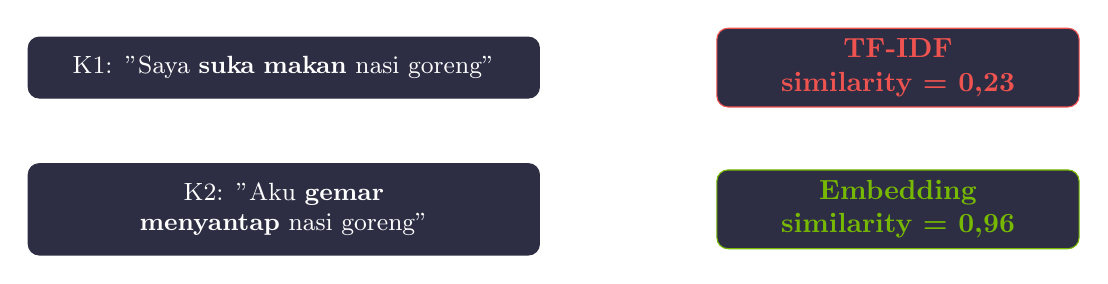
\begin{tikzpicture}[font=\small]
    \node[draw=nvcard, fill=nvcard, rounded corners=4pt, text=nvwhite,
          text width=6cm, align=center, inner sep=7pt] (k1) at (-3.6,1.6)
          {K1: "Saya \textbf{suka makan} nasi goreng"};
    \node[draw=nvcard, fill=nvcard, rounded corners=4pt, text=nvwhite,
          text width=6cm, align=center, inner sep=7pt] (k2) at (-3.6,-0.2)
          {K2: "Aku \textbf{gemar menyantap} nasi goreng"};
    \node[draw=nvred, fill=nvcard, rounded corners=4pt, text=nvred,
          font=\bfseries, minimum width=4.6cm, minimum height=1cm, align=center] (r) at (4.2,1.6)
          {TF-IDF\\similarity = 0,23};
    \node[draw=nvgreen, fill=nvcard, rounded corners=4pt, text=nvgreen,
          font=\bfseries, minimum width=4.6cm, minimum height=1cm, align=center] (g) at (4.2,-0.2)
          {Embedding\\similarity = 0,96};
  \end{tikzpicture}%
  }
  \end{center}
  \vspace{0.7em}
  \begin{itemize}
    \footnotesize
    \item Bagi TF-IDF, \texttt{suka} dan \texttt{gemar} adalah dua dimensi yang tidak berhubungan
    \item Yang tersisa hanya \texttt{nasi} dan \texttt{goreng} --- makanya skornya rendah
  \end{itemize}
  \vspace{0.2em}
  {\color{nvgray}\scriptsize Diukur di notebook 01 Section 9; \texttt{paraphrase-multilingual-MiniLM-L12-v2}.}
\end{frame}

\begin{frame}
  \intuisi{Embedding: makna sebagai koordinat}
  \vspace{0.3em}
  \begin{center}
  \resizebox{0.46\linewidth}{!}{%
  \begin{tikzpicture}[font=\small]
    \draw[->,color=nvgray] (-0.5,0) -- (7,0);
    \draw[->,color=nvgray] (0,-0.5) -- (0,4.6);
    % klaster makanan
    \draw[nvgreen, dashed, rounded corners] (0.7,2.6) rectangle (3.3,4.3);
    \node[text=nvgreen, font=\footnotesize] at (2.0,4.6) {makanan};
    \fill[nvgreen] (1.2,3.1) circle (0.11); \node[text=nvwhite, font=\tiny, right] at (1.3,3.1) {suka};
    \fill[nvgreen] (1.6,3.8) circle (0.11); \node[text=nvwhite, font=\tiny, right] at (1.7,3.8) {gemar};
    \fill[nvgreen] (2.4,3.3) circle (0.11); \node[text=nvwhite, font=\tiny, right] at (2.5,3.3) {menyantap};
    % klaster ekonomi
    \draw[nvorange, dashed, rounded corners] (4.6,0.6) rectangle (6.8,2.1);
    \node[text=nvorange, font=\footnotesize] at (5.7,2.4) {ekonomi};
    \fill[nvorange] (5.1,1.1) circle (0.11); \node[text=nvwhite, font=\tiny, right] at (5.2,1.1) {harga};
    \fill[nvorange] (5.6,1.7) circle (0.11); \node[text=nvwhite, font=\tiny, right] at (5.7,1.7) {BBM};
  \end{tikzpicture}%
  }
  \end{center}
  \vspace{0.3em}
  \begin{center}
    {\color{nvlightgreen}\small Kata bermakna mirip ditempatkan berdekatan, sehingga
    kemiripan makna bisa dihitung sebagai jarak.}
  \end{center}
\end{frame}

\begin{frame}{Satu Kalimat, 384 Angka}
  \begin{center}
  \resizebox{0.92\linewidth}{!}{%
  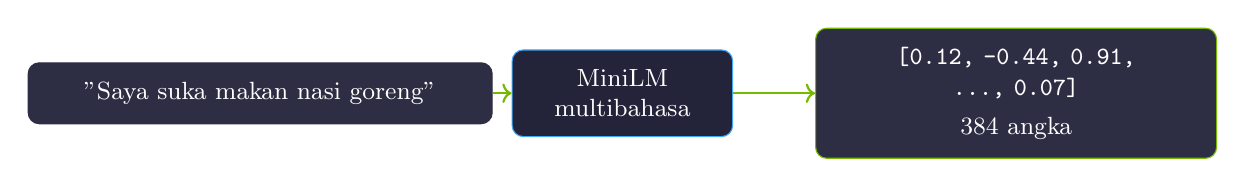
\begin{tikzpicture}[font=\small]
    \node[draw=nvcard, fill=nvcard, rounded corners=4pt, text=nvwhite,
          text width=5.4cm, align=center, inner sep=7pt] (in) at (-4.2,0)
          {"Saya suka makan nasi goreng"};
    \node[draw=nvblue, fill=nvdarkcard, rounded corners=4pt, text=nvwhite,
          minimum width=2.8cm, minimum height=1.1cm, align=center] (m) at (0.4,0)
          {MiniLM\\multibahasa};
    \node[draw=nvgreen, fill=nvcard, rounded corners=4pt, text=nvwhite,
          text width=4.6cm, align=center, inner sep=7pt] (out) at (5.4,0)
          {\texttt{[0.12, -0.44, 0.91,}\\\texttt{..., 0.07]}\\[3pt] 384 angka};
    \draw[->,thick,color=nvgreen] (in) -- (m);
    \draw[->,thick,color=nvgreen] (m) -- (out);
  \end{tikzpicture}%
  }
  \end{center}
  \vspace{0.7em}
  \begin{itemize}
    \footnotesize
    \item Panjang kalimat berapa pun selalu menghasilkan vektor sepanjang yang sama
    \item Model \texttt{paraphrase-multilingual-MiniLM-L12-v2} melayani puluhan bahasa sekaligus
    \item Karena multibahasa, kalimat Indonesia dan terjemahan Inggrisnya berdekatan
  \end{itemize}
\end{frame}

\begin{frame}{Cosine Similarity: Mengukur Kedekatan Arah}
  \begin{columns}[T]
    \begin{column}{0.46\textwidth}
      \begin{center}
      \resizebox{\linewidth}{!}{%
      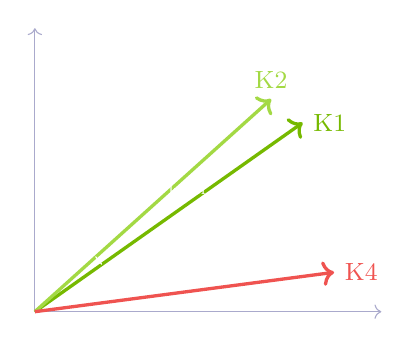
\begin{tikzpicture}[font=\small]
        \draw[->,color=nvgray] (0,0) -- (4.4,0);
        \draw[->,color=nvgray] (0,0) -- (0,3.6);
        \draw[->,very thick,color=nvgreen] (0,0) -- (3.4,2.4) node[right, text=nvgreen] {K1};
        \draw[->,very thick,color=nvlightgreen] (0,0) -- (3.0,2.7) node[above, text=nvlightgreen] {K2};
        \draw[->,very thick,color=nvred] (0,0) -- (3.8,0.5) node[right, text=nvred] {K4};
        \draw[color=nvwhite, thin] (0.85,0.6) arc (35:42:1.05);
        \node[text=nvwhite, font=\tiny] at (1.6,1.55) {sudut kecil};
      \end{tikzpicture}%
      }
      \end{center}
    \end{column}
    \begin{column}{0.5\textwidth}
      \begin{itemize}
        \footnotesize
        \item Mengukur \textbf{sudut} antar vektor, bukan panjangnya
        \item Nilai 1 = arah sama persis, 0 = tegak lurus (tidak berhubungan)
        \item Panjang diabaikan, jadi dokumen panjang dan pendek tetap adil dibandingkan
      \end{itemize}
      \vspace{0.4em}
      \begin{center}
      \nvbox{Di kode}{\footnotesize\texttt{cosine\_similarity(emb\_query, emb\_dokumen)}}
      \end{center}
    \end{column}
  \end{columns}
\end{frame}

\begin{frame}{Semantic Search dalam Sepuluh Baris}
  \begin{center}
  \resizebox{0.95\linewidth}{!}{%
  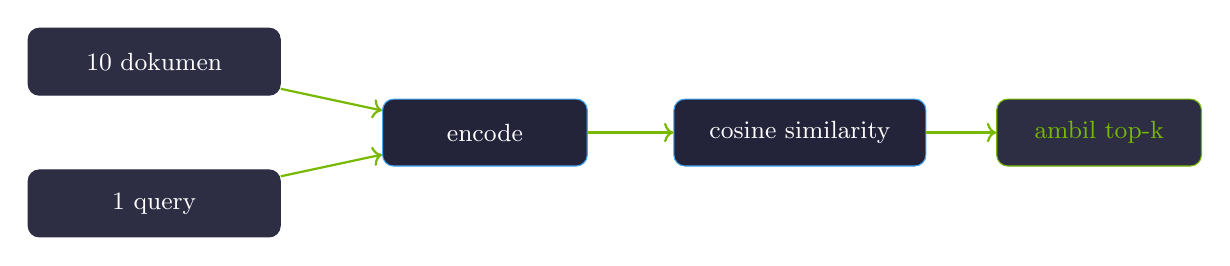
\begin{tikzpicture}[font=\small]
    \node[draw=nvcard, fill=nvcard, rounded corners=4pt, text=nvwhite,
          minimum width=3.2cm, minimum height=0.85cm, align=center] (d) at (0,1.5) {10 dokumen};
    \node[draw=nvcard, fill=nvcard, rounded corners=4pt, text=nvwhite,
          minimum width=3.2cm, minimum height=0.85cm, align=center] (q) at (0,-0.3) {1 query};
    \node[draw=nvblue, fill=nvdarkcard, rounded corners=4pt, text=nvwhite,
          minimum width=2.6cm, minimum height=0.85cm, align=center] (e) at (4.2,0.6) {encode};
    \node[draw=nvblue, fill=nvdarkcard, rounded corners=4pt, text=nvwhite,
          minimum width=3.2cm, minimum height=0.85cm, align=center] (c) at (8.2,0.6) {cosine similarity};
    \node[draw=nvgreen, fill=nvcard, rounded corners=4pt, text=nvgreen,
          minimum width=2.6cm, minimum height=0.85cm, align=center] (t) at (12.0,0.6) {ambil top-k};
    \draw[->,thick,color=nvgreen] (d) -- (e);
    \draw[->,thick,color=nvgreen] (q) -- (e);
    \draw[->,thick,color=nvgreen] (e) -- (c);
    \draw[->,thick,color=nvgreen] (c) -- (t);
  \end{tikzpicture}%
  }
  \end{center}
  \vspace{0.9em}
  \begin{beamercolorbox}[rounded=true,shadow=false,sep=6pt]{block body}
    \small\color{white}
    Query \textit{"puncak paling tinggi di Indonesia"} menemukan
    \textit{"Gunung Kerinci adalah gunung berapi tertinggi di Indonesia"} ---
    \textbf{tanpa satu pun kata yang sama}. TF-IDF tidak akan pernah menemukannya.
  \end{beamercolorbox}
\end{frame}

\begin{frame}{Inilah Inti RAG}
  \begin{center}
  \resizebox{0.9\linewidth}{!}{%
  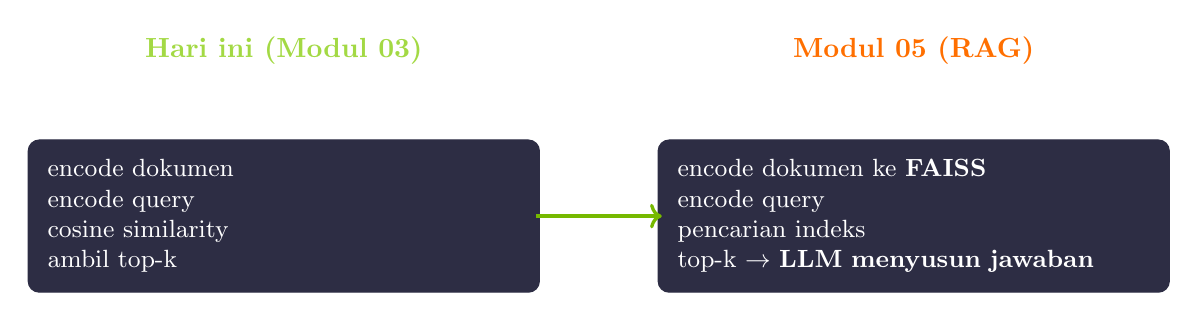
\begin{tikzpicture}[font=\small]
    \node[text=nvlightgreen, font=\bfseries] at (-3.6,2.5) {Hari ini (Modul 03)};
    \node[text=nvorange, font=\bfseries] at (4.4,2.5) {Modul 05 (RAG)};
    \node[draw=nvcard, fill=nvcard, rounded corners=4pt, text=nvwhite,
          text width=6cm, align=left, inner sep=7pt] (a) at (-3.6,0.4)
          {encode dokumen\\encode query\\cosine similarity\\ambil top-k};
    \node[draw=nvcard, fill=nvcard, rounded corners=4pt, text=nvwhite,
          text width=6cm, align=left, inner sep=7pt] (b) at (4.4,0.4)
          {encode dokumen ke \textbf{FAISS}\\encode query\\pencarian indeks\\top-k $\to$ \textbf{LLM menyusun jawaban}};
    \draw[->,very thick,color=nvgreen] (-0.4,0.4) -- (1.2,0.4);
  \end{tikzpicture}%
  }
  \end{center}
  \vspace{0.7em}
  \begin{itemize}
    \footnotesize
    \item Polanya identik --- yang bertambah hanya indeks agar cepat untuk jutaan dokumen,
          dan LLM di ujung untuk menyusun kalimat jawaban
    \item Kamu sudah membangun bagian intinya hari ini
  \end{itemize}
\end{frame}

\begin{frame}[fragile]{Tokenisasi Subword: Token ala LLM}
  \begin{lstlisting}[language=Python]
tok = AutoTokenizer.from_pretrained("gpt2")
tok.tokenize("mempelajari")
# ['mem', 'pel', 'aj', 'ari']  -- potongan subword
  \end{lstlisting}
  \vspace{0.3em}
  \begin{itemize}
    \footnotesize
    \item Potongan lebih kecil dari kata, lebih besar dari huruf
    \item Kosakata terbatas ($\sim$30--50 ribu subword) bisa menuliskan kata apa pun,
          termasuk yang belum pernah dilihat saat training
    \item Untuk bahasa Indonesia yang kaya imbuhan, \texttt{mempelajari} dan
          \texttt{dipelajari} berbagi potongan yang sama
  \end{itemize}
\end{frame}

\begin{frame}
  \intuisi{Token adalah satuan biaya}
  \vspace{0.4em}
  \begin{center}
  \resizebox{0.85\linewidth}{!}{%
  
\begin{tikzpicture}[font=\small]
    \node[text=nvwhite, font=\footnotesize] at (0,3.0) {dua pasang kalimat semakna, tokenizer GPT-2};
    \node[text=nvwhite, font=\footnotesize, left] at (-4.2,2.0) {Inggris};
    \fill[nvgreen] (-4.0,1.8) rectangle (-1.2,2.2);
    \node[text=nvwhite, font=\footnotesize, right] at (-1.0,2.0) {16 token};
    \node[text=nvwhite, font=\footnotesize, left] at (-4.2,1.0) {Indonesia};
    \fill[nvorange] (-4.0,0.8) rectangle (3.0,1.2);
    \node[text=nvwhite, font=\footnotesize, right] at (3.2,1.0) {40 token \ (2,50x)};
  \end{tikzpicture}%
  }
  \end{center}
  \vspace{0.5em}
  \begin{itemize}
    \footnotesize
    \item Tokenizer GPT-2 dilatih dominan pada teks Inggris, jadi kata Indonesia terpecah lebih halus
    \item API LLM menagih \textbf{per token} --- kalimat Indonesia jadi lebih mahal untuk isi yang sama
    \item Tokenizer multibahasa menekan rasio itu jadi 1,35x pada dua kalimat yang sama
  \end{itemize}
  \vspace{0.2em}
  {\color{nvgray}\scriptsize Diukur di notebook 01 Section 10; hitung ulang dengan kalimatmu sendiri.}
\end{frame}

\begin{frame}{"Token" Mulai Modul 04}
  \begin{center}
  \renewcommand{\arraystretch}{1.3}
  {\footnotesize
  \begin{tabular}{@{}p{0.30\linewidth}p{0.28\linewidth}p{0.34\linewidth}@{}}
    \toprule
    \rowcolor{nvcard!50}
    \textbf{Konteks} & \textbf{Satu token =} & \textbf{Dipakai di} \\
    \midrule
    Bagian A modul ini & satu kata & \texttt{tokenizer.tokenize()} \\
    Bagian D modul ini & satu subword & \texttt{AutoTokenizer} \\
    Modul 04 dan seterusnya & satu subword & \texttt{max\_new\_tokens}, batas konteks, tagihan API \\
    \bottomrule
  \end{tabular}%
  }
  \end{center}
  \vspace{0.9em}
  \begin{center}
    {\color{nvlightgreen}\small Mulai besok, kata "token" selalu berarti subword.}
  \end{center}
\end{frame}

\begin{frame}{Ringkasan Act 5}
  \begin{itemize}
    \item[\textcolor{nvgreen}{\checkmark}] TF-IDF membobot kata langka lebih tinggi, tetapi tetap mencocokkan ejaan
    \item[\textcolor{nvgreen}{\checkmark}] Embedding memetakan makna jadi koordinat --- sinonim berdekatan
    \item[\textcolor{nvgreen}{\checkmark}] Cosine similarity mengukur sudut, sehingga panjang dokumen tidak mengganggu
    \item[\textcolor{nvgreen}{\checkmark}] Semantic search = encode, bandingkan, ambil top-k --- inti RAG
    \item[\textcolor{nvgreen}{\checkmark}] Tokenisasi subword menentukan biaya sebuah bahasa di API LLM
  \end{itemize}
  \vspace{0.9em}
  \begin{center}
    {\color{nvlightgreen}\small Semua ini berjalan di CPU. Act 6 menjalankan alur yang sama di GPU.}
  \end{center}
\end{frame}

% ============================================================
% ACT 6 — NLP DI GPU
% ============================================================
\acttitle{6}{NLP di GPU}{NVIDIA RAPIDS --- alur yang sama, skala yang berbeda}

\begin{frame}{Kenapa NLP Klasik Butuh GPU}
  \begin{columns}[T]
    \begin{column}{0.5\textwidth}
      \begin{itemize}
        \footnotesize
        \item Menyiapkan korpus LLM berarti memproses \textbf{miliaran} dokumen
        \item Operasi teks bersifat seragam dan berulang --- persis yang disukai ribuan core GPU
        \item Preprocessing yang butuh berjam-jam di CPU bisa selesai dalam hitungan menit
      \end{itemize}
    \end{column}
    \begin{column}{0.46\textwidth}
      \begin{center}
      \resizebox{\linewidth}{!}{%
      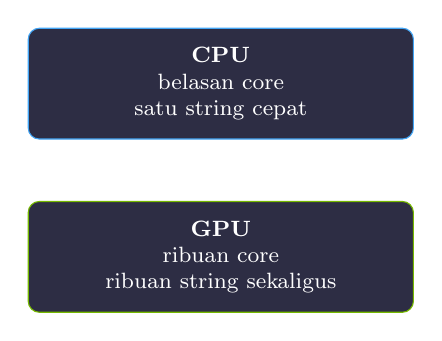
\begin{tikzpicture}[font=\footnotesize]
        \node[draw=nvblue, fill=nvcard, rounded corners=4pt, text=nvwhite,
              text width=4.4cm, align=center, inner sep=7pt] (c) at (0,1.3)
              {\textbf{CPU}\\belasan core\\satu string cepat};
        \node[draw=nvgreen, fill=nvcard, rounded corners=4pt, text=nvwhite,
              text width=4.4cm, align=center, inner sep=7pt] (g) at (0,-0.9)
              {\textbf{GPU}\\ribuan core\\ribuan string sekaligus};
      \end{tikzpicture}%
      }
      \end{center}
    \end{column}
  \end{columns}
  \vspace{0.6em}
  \centering\footnotesize\textcolor{nvgray}{Praktik: notebook \texttt{02\_nlp\_on\_steroids}}
\end{frame}

\begin{frame}{Stack RAPIDS untuk NLP}
  \begin{center}
  \renewcommand{\arraystretch}{1.3}
  {\footnotesize
  \begin{tabular}{@{}p{0.18\linewidth}p{0.34\linewidth}p{0.40\linewidth}@{}}
    \toprule
    \rowcolor{nvcard!50}
    \textbf{Library} & \textbf{Padanan CPU} & \textbf{Peran} \\
    \midrule
    \texttt{cuDF} & \texttt{pandas} & DataFrame di memori GPU \\
    \texttt{nvtext} & --- & Operasi teks GPU: \texttt{tokenize}, \texttt{ngrams\_tokenize}, \texttt{minhash} \\
    \texttt{cuML} & \texttt{scikit-learn} & TF-IDF, Logistic Regression, clustering \\
    \bottomrule
  \end{tabular}%
  }
  \end{center}
  \vspace{0.8em}
  \begin{itemize}
    \footnotesize
    \item Sudah terpasang di runtime GPU Colab --- tinggal \texttt{import}
    \item \texttt{nvtext} tidak punya padanan di pandas: operasinya memang lahir di GPU
  \end{itemize}
\end{frame}

\begin{frame}[fragile]{Nol Perubahan Kode: cudf.pandas \& cuml.accel}
  \begin{lstlisting}
# CPU: pandas + sklearn biasa
python pipeline.py

# GPU: file yang SAMA, nol perubahan kode
python -m cudf.pandas -m cuml.accel pipeline.py
  \end{lstlisting}
  \vspace{0.4em}
  \begin{itemize}
    \footnotesize
    \item \texttt{cudf.pandas} mengambil alih \texttt{import pandas} dan mengalihkan operasinya ke GPU
    \item \texttt{cuml.accel} melakukan hal yang sama untuk estimator scikit-learn
    \item Operasi yang belum didukung GPU otomatis \emph{fallback} ke CPU --- kode tidak crash
    \item Akurasi identik; yang berubah hanya \textbf{waktu}
  \end{itemize}
\end{frame}

\begin{frame}
  \intuisi{GPU tidak selalu menang}
  \vspace{0.4em}
  \begin{center}
  \resizebox{0.85\linewidth}{!}{%
  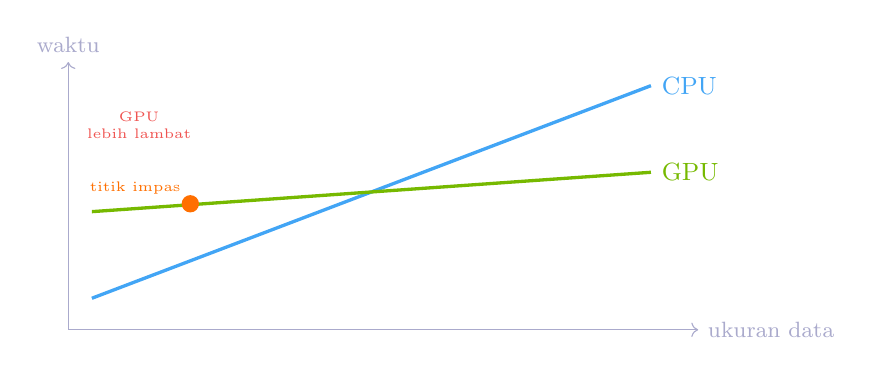
\begin{tikzpicture}[font=\small]
    \draw[->,color=nvgray] (0,0) -- (8,0) node[right, text=nvgray, font=\footnotesize] {ukuran data};
    \draw[->,color=nvgray] (0,0) -- (0,3.4) node[above, text=nvgray, font=\footnotesize] {waktu};
    \draw[very thick, color=nvblue] (0.3,0.4) -- (7.4,3.1) node[right, text=nvblue] {CPU};
    \draw[very thick, color=nvgreen] (0.3,1.5) -- (7.4,2.0) node[right, text=nvgreen] {GPU};
    \fill[nvorange] (1.55,1.6) circle (0.11);
    \node[text=nvorange, font=\tiny, above left] at (1.55,1.6) {titik impas};
    \node[text=nvred, font=\tiny, align=center] at (0.9,2.6) {GPU\\lebih lambat};
  \end{tikzpicture}%
  }
  \end{center}
  \vspace{0.4em}
  \begin{itemize}
    \footnotesize
    \item GPU membayar biaya tetap: inisialisasi CUDA dan pemindahan data CPU$\leftrightarrow$GPU
    \item Untuk data kecil, biaya tetap itu lebih mahal daripada komputasinya sendiri
    \item \textbf{Aturan emas benchmark:} jangan pernah mengukur pemanggilan GPU pertama --- lakukan \emph{warm-up} dulu
  \end{itemize}
\end{frame}

\begin{frame}{nvtext: Operasi yang Tidak Ada di pandas}
  \begin{center}
  \renewcommand{\arraystretch}{1.3}
  {\footnotesize
  \begin{tabular}{@{}p{0.34\linewidth}p{0.58\linewidth}@{}}
    \toprule
    \rowcolor{nvcard!50}
    \textbf{Operasi} & \textbf{Gunanya} \\
    \midrule
    \texttt{str.token\_count()} & Hitung token per baris tanpa membentuk daftar \\
    \texttt{str.tokenize()} & Pecah seluruh kolom jadi token sekaligus \\
    \texttt{str.ngrams\_tokenize(2)} & Bangun bigram langsung di GPU \\
    \texttt{str.minhash()} & Sidik jari dokumen untuk deteksi duplikat \\
    \bottomrule
  \end{tabular}%
  }
  \end{center}
  \vspace{0.8em}
  \begin{center}
    {\color{nvlightgreen}\small Makin intensif operasi string-nya, makin lebar kemenangan GPU ---
    karena ribuan core mengerjakan ribuan baris serentak.}
  \end{center}
\end{frame}

\begin{frame}{Seberapa Cepat? (Colab T4, 150 ribu paragraf Wikipedia ID)}
  \begin{center}
    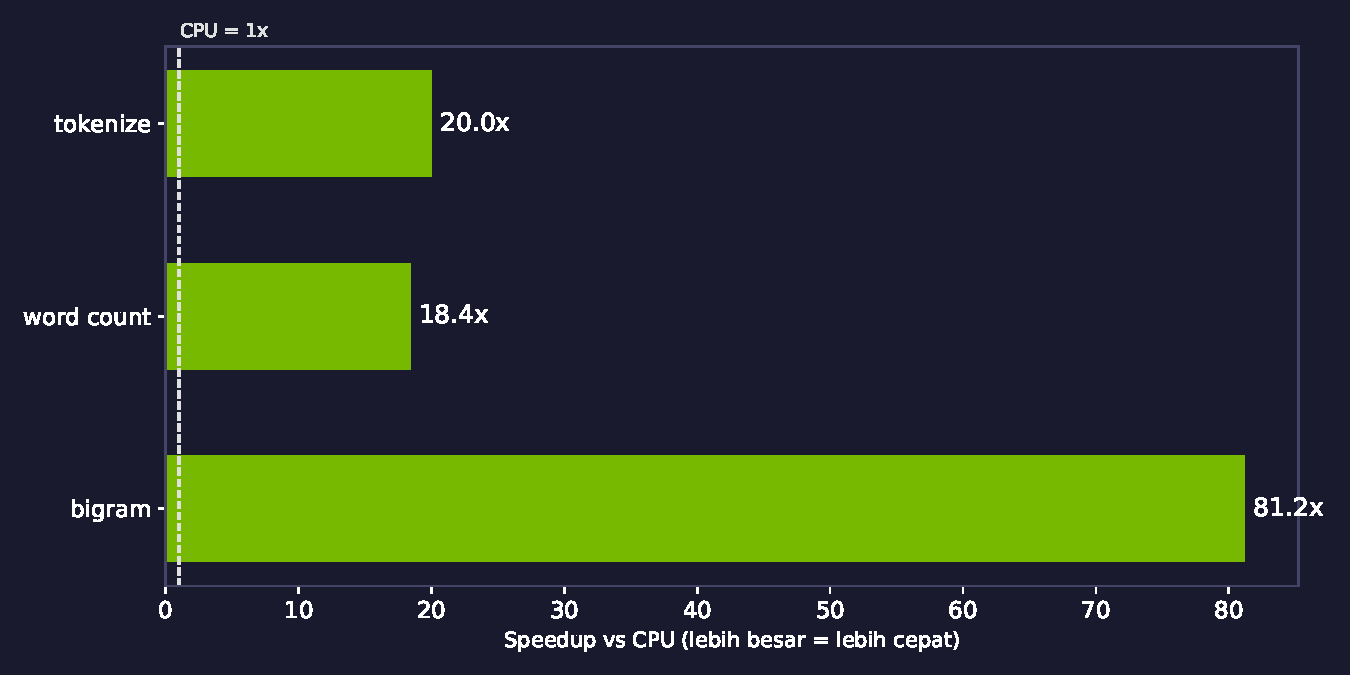
\includegraphics[width=0.88\textwidth]{figures/rapids_speedup.pdf}
  \end{center}
  \footnotesize\textcolor{nvgray}{Diukur langsung di notebook \texttt{02\_nlp\_on\_steroids} --- angka di mesinmu bisa berbeda.}
\end{frame}

\begin{frame}{MinHash: Dari Miliaran Perbandingan Jadi Satu groupby}
  \begin{center}
  \resizebox{0.92\linewidth}{!}{%
  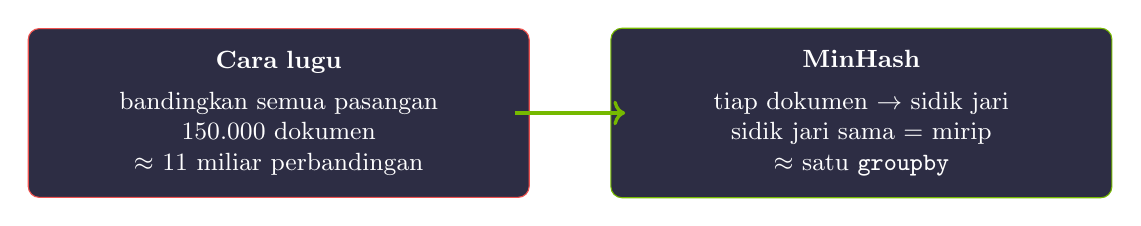
\begin{tikzpicture}[font=\small]
    \node[draw=nvred, fill=nvcard, rounded corners=4pt, text=nvwhite,
          text width=5.8cm, align=center, inner sep=8pt] (a) at (-3.6,0)
          {\textbf{Cara lugu}\\[4pt]
           bandingkan semua pasangan\\
           150.000 dokumen\\
           $\approx$ 11 miliar perbandingan};
    \node[draw=nvgreen, fill=nvcard, rounded corners=4pt, text=nvwhite,
          text width=5.8cm, align=center, inner sep=8pt] (b) at (3.8,0)
          {\textbf{MinHash}\\[4pt]
           tiap dokumen $\to$ sidik jari\\
           sidik jari sama = mirip\\
           $\approx$ satu \texttt{groupby}};
    \draw[->,very thick,color=nvgreen] (-0.6,0) -- (0.8,0);
  \end{tikzpicture}%
  }
  \end{center}
  \vspace{0.7em}
  \begin{itemize}
    \footnotesize
    \item Duplikat di korpus training berarti model menghafal dan komputasi terbuang
    \item Notebook memakai satu sidik jari utuh, jadi hanya duplikat nyaris identik yang tertangkap
    \item Sistem produksi (MinHash-LSH) memakai banyak \emph{band} agar kemiripan parsial ikut terdeteksi
  \end{itemize}
\end{frame}

\begin{frame}
  \intuisi{Kenapa sidik jari bisa menggantikan perbandingan}
  \vspace{0.5em}
  \begin{center}
  \resizebox{0.9\linewidth}{!}{%
  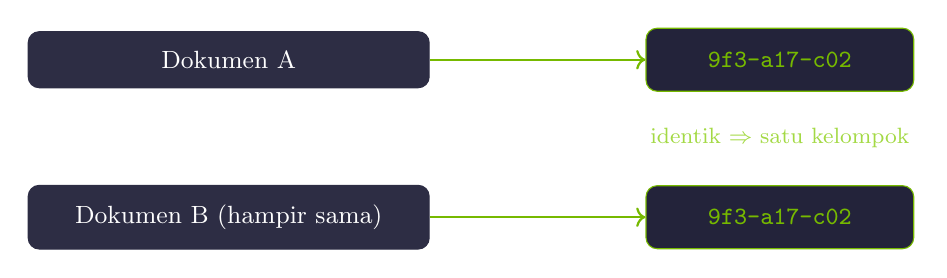
\begin{tikzpicture}[font=\small]
    \node[draw=nvcard, fill=nvcard, rounded corners=4pt, text=nvwhite,
          text width=4.6cm, align=center, inner sep=7pt] (d1) at (-4.4,1.4)
          {Dokumen A};
    \node[draw=nvcard, fill=nvcard, rounded corners=4pt, text=nvwhite,
          text width=4.6cm, align=center, inner sep=7pt] (d2) at (-4.4,-0.6)
          {Dokumen B (hampir sama)};
    \node[draw=nvgreen, fill=nvdarkcard, rounded corners=4pt, text=nvgreen,
          minimum width=3.4cm, minimum height=0.8cm] (h1) at (2.6,1.4) {\texttt{9f3-a17-c02}};
    \node[draw=nvgreen, fill=nvdarkcard, rounded corners=4pt, text=nvgreen,
          minimum width=3.4cm, minimum height=0.8cm] (h2) at (2.6,-0.6) {\texttt{9f3-a17-c02}};
    \draw[->,thick,color=nvgreen] (d1) -- (h1);
    \draw[->,thick,color=nvgreen] (d2) -- (h2);
    \node[text=nvlightgreen, font=\footnotesize] at (2.6,0.4) {identik $\Rightarrow$ satu kelompok};
  \end{tikzpicture}%
  }
  \end{center}
  \vspace{0.6em}
  \begin{center}
    {\color{nvlightgreen}\small Dokumen mirip menghasilkan sidik jari sama dengan probabilitas tinggi.
    Masalah "cari yang mirip" berubah jadi "kelompokkan yang sama" --- dan yang kedua jauh lebih murah.}
  \end{center}
\end{frame}

\begin{frame}{Dari Lab ke Produksi: NeMo Curator}
  \begin{center}
  \renewcommand{\arraystretch}{1.3}
  {\footnotesize
  \begin{tabular}{@{}p{0.44\linewidth}p{0.48\linewidth}@{}}
    \toprule
    \rowcolor{nvcard!50}
    \textbf{Hari ini (1 T4, 150 ribu paragraf)} & \textbf{Produksi (ratusan GPU, miliaran dokumen)} \\
    \midrule
    \texttt{tokenize}, \texttt{normalize} di nvtext & Identifikasi bahasa, pembersihan, penyaringan kualitas \\
    MinHash + \texttt{groupby} & Fuzzy dedup MinHash-LSH terdistribusi \\
    TF-IDF + Logistic Regression & Classifier kualitas dokumen \\
    \bottomrule
  \end{tabular}%
  }
  \end{center}
  \vspace{0.8em}
  \begin{center}
    {\color{nvlightgreen}\small Bedanya cuma skala. Langkah-langkahnya sama persis dengan yang kamu jalankan hari ini.}
  \end{center}
\end{frame}

\begin{frame}{Ringkasan Act 6}
  \begin{itemize}
    \item[\textcolor{nvgreen}{\checkmark}] \texttt{cudf.pandas} dan \texttt{cuml.accel} memindahkan kode lama ke GPU tanpa mengubahnya
    \item[\textcolor{nvgreen}{\checkmark}] \texttt{nvtext} menyediakan operasi teks yang tidak ada padanannya di pandas
    \item[\textcolor{nvgreen}{\checkmark}] GPU menang di skala; untuk data kecil ia justru bisa lebih lambat
    \item[\textcolor{nvgreen}{\checkmark}] Warm-up wajib sebelum mengukur apa pun di GPU
    \item[\textcolor{nvgreen}{\checkmark}] MinHash mengubah masalah kuadratik jadi satu \texttt{groupby}
  \end{itemize}
  \vspace{0.9em}
  \begin{center}
    {\color{nvlightgreen}\small Peta library NVIDIA: RAPIDS hari ini, NeMo dan TensorRT-LLM di Modul 06.}
  \end{center}
\end{frame}

% ============================================================
% ACT 7 — RINGKASAN & LANJUTAN
% ============================================================
\acttitle{7}{Ringkasan \& Lanjutan}{Apa yang dibawa pulang, dan apa berikutnya}

\begin{frame}{Ringkasan Modul 03}
  \begin{center}
  \renewcommand{\arraystretch}{1.05}
  {\scriptsize
  \begin{tabular}{@{}p{0.06\linewidth}p{0.05\linewidth}p{0.34\linewidth}p{0.45\linewidth}@{}}
    \toprule
    \rowcolor{nvcard!50}
    \textbf{Bag.} & \textbf{\#} & \textbf{Topik} & \textbf{Yang dikuasai} \\
    \midrule
    A & 1 & Pipeline pra-pemrosesan & Teks mentah jadi token bersih \\
    A & 2 & POS tagging & Menandai kelas kata \\
    A & 3 & Tokenisasi frasa & Entitas multi-kata tetap utuh \\
    A & 4 & Stopword \& lemmatisasi & Menekan kata umum, kembalikan bentuk dasar \\
    B & 5 & Frekuensi kata & Menebak topik, word cloud vs bar chart \\
    B & 6 & NER & Teks bebas jadi data terstruktur \\
    C & 7 & Sentimen & Leksikon vs transformer (IndoBERT) \\
    C & 8 & Klasifikasi Naive Bayes & Bag-of-words tanpa kebocoran data \\
    D & 9 & Kata ke vektor & TF-IDF, embedding, semantic search \\
    D & 10 & Tokenisasi subword & Arti "token" mulai Modul 04 \\
    \midrule
    \multicolumn{2}{@{}l}{\textbf{NB 02}} & NLP di GPU & RAPIDS, nvtext, MinHash, benchmark jujur \\
    \bottomrule
  \end{tabular}%
  }
  \end{center}
\end{frame}

\begin{frame}{Tiga Hal yang Dibawa Pulang}
  \begin{columns}[T]
    \begin{column}{0.32\textwidth}
      \nvbox{1. Pembersihan menentukan}{\footnotesize Tanpa membuang stopword,
      analisis frekuensi apa pun hanya memunculkan \texttt{yang} dan \texttt{di}.}
    \end{column}
    \begin{column}{0.32\textwidth}
      \nvbox{2. Fit hanya pada train}{\footnotesize Daftar fitur, vectorizer, scaler.
      Melanggarnya tidak memberi error --- hanya akurasi palsu.}
    \end{column}
    \begin{column}{0.32\textwidth}
      \nvbox{3. Hitungan $\neq$ makna}{\footnotesize TF-IDF buta terhadap sinonim,
      embedding tidak. Perbedaan itulah yang membuat RAG mungkin.}
    \end{column}
  \end{columns}
\end{frame}

\begin{frame}{Notebook 01: Peta Section}
  \begin{columns}[T]
    \begin{column}{0.48\textwidth}
      \textcolor{nvgreen}{\textbf{Isi:}}
      \begin{itemize}
        \footnotesize
        \item Bagian A --- pembersihan teks (Section 1--4)
        \item Bagian B --- frekuensi \& NER (Section 5--6)
        \item Bagian C --- sentimen \& klasifikasi (Section 7--8)
        \item Bagian D --- vektor \& subword (Section 9--10)
        \item Latihan: 4 soal
      \end{itemize}
    \end{column}
    \begin{column}{0.48\textwidth}
      \textcolor{nvlightgreen}{\textbf{Library:}}
      \begin{itemize}
        \footnotesize
        \item \texttt{nlp-id} --- tokenizer, POS, stopword, lemmatizer
        \item \texttt{nltk} --- korpus \texttt{movie\_reviews}, Naive Bayes
        \item \texttt{spaCy} --- NER Inggris
        \item \texttt{textblob} --- sentimen leksikon
        \item \texttt{sentence-transformers} --- embedding
        \item \texttt{transformers} --- IndoBERT, tokenizer subword
      \end{itemize}
    \end{column}
  \end{columns}
  \vspace{0.5em}
  \begin{beamercolorbox}[rounded=true,shadow=false,sep=4pt]{block body}
    \small\color{white}
    \textbf{Runtime}: CPU cukup \quad $\cdot$ \quad \textbf{Estimasi}: $\pm$ 60 menit
  \end{beamercolorbox}
\end{frame}

\begin{frame}{Notebook 02: Peta Babak}
  \begin{columns}[T]
    \begin{column}{0.48\textwidth}
      \textcolor{nvorange}{\textbf{Isi:}}
      \begin{itemize}
        \footnotesize
        \item Babak 1 --- nol perubahan kode di GPU
        \item Babak 2 --- nvtext pada 150 ribu paragraf Wikipedia
        \item Babak 3 --- dedup MinHash
        \item Babak 4 --- cuML native + pelajaran warm-up
        \item Babak 5 --- NeMo Curator dan jembatan ke LLM
      \end{itemize}
    \end{column}
    \begin{column}{0.48\textwidth}
      \textcolor{nvlightgreen}{\textbf{Data:}}
      \begin{itemize}
        \footnotesize
        \item SmSA (IndoNLU) --- ulasan Indonesia berlabel sentimen
        \item Wikipedia Bahasa Indonesia via streaming
      \end{itemize}
    \end{column}
  \end{columns}
  \vspace{0.5em}
  \begin{beamercolorbox}[rounded=true,shadow=false,sep=4pt]{block body}
    \small\color{white}
    \textbf{Runtime}: wajib T4 GPU \quad $\cdot$ \quad \textbf{Estimasi}: $\pm$ 45 menit
  \end{beamercolorbox}
\end{frame}

\begin{frame}[fragile]{Setup \& Tools}
  \begin{columns}[T]
    \begin{column}{0.5\textwidth}
      \textcolor{nvgreen}{\textbf{Notebook 01 (CPU):}}
      \begin{lstlisting}[language=bash, basicstyle=\ttfamily\scriptsize\color{nvwhite}]
!pip install "nlp-id>=0.1.23,<0.2" \
  "transformers>=5,<6" \
  "sentence-transformers>=5,<6"
!python -m spacy download en_core_web_sm
      \end{lstlisting}
    \end{column}
    \begin{column}{0.46\textwidth}
      \textcolor{nvorange}{\textbf{Yang mudah salah:}}
      \begin{itemize}
        \footnotesize
        \item \texttt{nlp-id} mengunci \texttt{huggingface-hub 1.x}, jadi \texttt{transformers} harus 5.x
        \item Colab minta \textbf{restart session} setelah instalasi --- lakukan, jangan ulangi \texttt{pip}
        \item Notebook 02 butuh runtime \textbf{T4 GPU}; RAPIDS sudah terpasang
      \end{itemize}
    \end{column}
  \end{columns}
\end{frame}

\begin{frame}{Lanjutan: Modul 04 -- LLM}
  \begin{itemize}
    \item[\textcolor{nvgreen}{\checkmark}] \textbf{Modul 04} --- Large Language Models: \texttt{pipeline} dari Section 7
          dan "token" dari Section 10 jadi pintu masuknya
    \item[\textcolor{nvgreen}{\checkmark}] \textbf{Modul 05} --- RAG: pola embedding + semantic search dari Section 9,
          kali ini dengan FAISS
    \item[\textcolor{nvgreen}{\checkmark}] \textbf{Modul 06} --- Ekosistem NVIDIA: NeMo dan TensorRT-LLM,
          lanjutan langsung dari RAPIDS hari ini
  \end{itemize}
  \vspace{0.8em}
  \begin{center}
  \resizebox{0.7\linewidth}{!}{%
  
\begin{tikzpicture}
    \node[draw=nvgreen, fill=nvcard, rounded corners=6pt,
          text=white, font=\small, minimum width=2.2cm, minimum height=0.8cm,
          align=center] (nlp) at (0,0) {NLP\\(kita di sini)};
    \node[draw=nvcard, fill=nvcard, rounded corners=6pt,
          text=white, font=\small, minimum width=2.2cm, minimum height=0.8cm,
          align=center] (llm) at (3,0) {LLM\\(berikutnya)};
    \node[draw=nvcard, fill=nvcard, rounded corners=6pt,
          text=white, font=\small, minimum width=2.2cm, minimum height=0.8cm,
          align=center] (rag) at (6,0) {RAG};
    \draw[->,thick,color=nvgreen] (nlp) -- (llm);
    \draw[->,thick,color=nvgreen] (llm) -- (rag);
  \end{tikzpicture}%
  }
  \end{center}
\end{frame}

\begin{frame}[plain]
  \vspace{2cm}
  \begin{center}
    {\color{nvgreen}\Huge\bfseries Terima Kasih!}\\[1.5em]
    {\color{nvgray}\Large Pertanyaan? Diskusi?}\\[2em]
    \begin{beamercolorbox}[rounded=true,shadow=false,sep=8pt,wd=10cm]{block body}
      \centering\color{white}
      \textbf{NLP Fundamentals} \quad $\cdot$ \quad Modul 03 \\
      Navasena Gen-ML Course
    \end{beamercolorbox}
  \end{center}
\end{frame}

\end{document}
